

\documentclass[oneside,11pt]{article}


\usepackage{soul}
\usepackage{natbib}
\usepackage{hyperref}
\usepackage{bookmark}
\usepackage{graphicx}             
\graphicspath{{./Figuras/}}
\usepackage{enumitem}

\usepackage{makecell}
\usepackage[margin=1in]{geometry}
\usepackage{float}                
\usepackage{amsmath}

\usepackage{amsfonts}       %enrique
\usepackage{amsmath,amssymb} %enrique
\usepackage{amscd}
\usepackage{amsfonts}
\usepackage{amssymb}
\usepackage{bbm}
\usepackage{booktabs}
\usepackage{nameref}
\usepackage{multirow}
\usepackage[nokeyprefix]{refstyle}
\usepackage{rotating}
\usepackage{threeparttable}
\usepackage{afterpage}
\usepackage{lscape}
\usepackage{caption}
\usepackage{subcaption}
\usepackage{epstopdf}
\usepackage{setspace}
\usepackage{svg}
\usepackage{dsfont}
\usepackage{amsthm}
\usepackage{tocloft}
\usepackage{etoc}
\usepackage{lmodern}
\usepackage{bm}
\usepackage{tablefootnote}
\usepackage{longtable}
\usepackage[colorinlistoftodos,prependcaption,textsize=tiny]{todonotes}

\epstopdfDeclareGraphicsRule{.tiff}{png}{.png}{convert #1 \OutputFile}
\AppendGraphicsExtensions{.tiff}

\epstopdfDeclareGraphicsRule{.tif}{png}{.png}{convert #1 \OutputFile}
\AppendGraphicsExtensions{.tif}

\usepackage{tikz}
\usetikzlibrary{shapes.geometric, arrows}
\usetikzlibrary{calc}
\usetikzlibrary{matrix}

\tikzset{ 
    table/.style={
        matrix of nodes,
        row sep=-\pgflinewidth,
        column sep=-\pgflinewidth,
        nodes={
            rectangle,
            draw=black,
            align=center
        },
        minimum height=1.5em,
        text depth=0.5ex,
        text height=2ex,
        nodes in empty cells,
%%
        every even row/.style={
            nodes={fill=gray!20}
        },
        column 1/.style={
            nodes={text width=2em,font=\bfseries}
        },
        row 1/.style={
            nodes={
                fill=black,
                text=white,
                font=\bfseries
            }
        }
    }
}


\usepackage{colortbl}

\newtheorem{theorem}{Theorem}
\newtheorem{claim}[theorem]{Claim}
\newtheorem{prop}[theorem]{Proposition} 
\newtheorem{cor}[theorem]{Corollary} 
\newtheorem{assumption}{Assumption} 
\newtheorem{lem}{Lemma} 

\DeclareRobustCommand{\hlgr}[1]{{\sethlcolor{green}\hl{#1}}}


\usepackage{comment}
%para esconder columnas en tablas (enrique)
\usepackage{array}
\newcolumntype{H}{>{\setbox0=\hbox\bgroup}c<{\egroup}@{}}
\linespread{1.5}

\newcommand{\wh}{\widehat}
\usepackage{anyfontsize}

\usepackage[linesnumbered,vlined,ruled,commentsnumbered]{algorithm2e}

\DontPrintSemicolon
\newcommand{\To}{\mbox{\upshape\bfseries to}}
\newcommand{\E}{\mathbb{E}}

%%% HELPER CODE FOR DEALING WITH EXTERNAL REFERENCES
\usepackage{xr}
\makeatletter
\newcommand*{\addFileDependency}[1]{
  \typeout{(#1)}
  \@addtofilelist{#1}
  \IfFileExists{#1}{}{\typeout{No file #1.}}
}
\makeatother


\newcommand*{\myexternaldocument}[1]{
    \externaldocument{#1}
    \addFileDependency{#1.tex}
    \addFileDependency{#1.aux}
}

%\myexternaldocument{OA}

%%%%%%%%%%%%%%%%%%%%%%%%%%%%%%%% DOCUMENT
\begin{document}


\title{Did Seguro Popular Reduce Formal Jobs?  \thanks{We want to thank IMSS and WIEGO for support in getting data and financing for this project. We also want to thank Roberto Gonzalez Tellez and Luis Alberto Martinez Chigo  for excellent research assistance.}}
\author{Enrique Seira  \and Isaac Meza  \and Eduardo González-Pier \and Eduardo Alcaraz %\thanks{Seira: ITAM, enrique.seira@itam.mx;  González-Pier: Palladium and Wilson Center, eduardo.gonzalezpier@thepalladiumgroup.com; Meza: Harvard Economics, isaacmezalopez@g.harvard.edu; Alcaraz: IMSS.} 
}
\date{This draft:  \today \\[2 cm]}

%\vspace{.5in}


\maketitle
\thispagestyle{empty}
\begin{abstract}

Prominent international institutions have written that social protection benefits which are tied to not having formal employment make informal employment more attractive, and thus reduce formal employment by shifting workers to the informal sector. While the argument is simple and consistent, the question is an empirical one and evidence around it is scarce. We assess this hypothesis by studying Mexico's Seguro Popular (SP). SP has been at the forefront of this debate both because of its large size covering half of the population and close to 50 million people, but also since it has often been portrayed as the leading example of an informality inducing social policy. This document uses the roll-out of Mexico's SP across municipalities to quantitatively assess its impact on private sector formal employment in Mexico, using more detailed data and improved econometric methods compared to previous papers. We find no robust evidence of a decrease in formal employment, suggesting the attraction of SP was not large enough to overcome the benefits of having a formal job. We also find no effects in average salaries of jobs affiliated to IMSS, further suggesting that there were no strong shifts in labour supply from the formal to the informal sector. We need more work on the benefit side of SP, as the benefit side should be considered in an assessment of SP welfare consequences.


\end{abstract}

\vspace{.3in}


\newpage

\pagenumbering{arabic}
\etocdepthtag.toc{mtchapter}
\etocsettagdepth{mtchapter}{subsection}
\etocsettagdepth{mtappendix}{none}



\section{Introduction}

According to the International Labour Organization (ILO) 
``Two billion people – more than 61 per cent of the world’s employed population – make their living in the informal economy'' \citep{ILO_2018}. Most of them do not have access to social protection programs to insure against risks like unemployment and health shocks. The ILO calculates that just 47 per cent of the global population was effectively covered by at least one social protection benefit. This seems to be both unfair and inefficient. It works against basic social justice requirements \citep{Dworkin}, and it exposes workers to financial and productivity risks derived from health and labour hazards \citep{FoodStamps}. The COVID pandemic has been a highly regressive dual income and health shock.  The increased unemployment from disrupted labour markets and  higher mortality weighted more heavily among low income populations, most of them not covered by health insurance.  The pandemic has become a stark reminder of the need for stronger more inclusive social protection mechanisms \citep{Arceo_Covid, COVID_gap_US}.

Policy makers and international institutions often focus on the cost of social protection policies, not only in terms of fiscal burdens, but specifically on the claim that they shift jobs from the formal to the informal sector of the economy \citep{Levy_2008,UNDP}. The argument is that social protection systems which combine employment-linked social insurance with tax-financed social assistance for low-income informal workers increase informality because they increase the cost of creating a formal job relative to an informal one. Moreover, from a worker perspective, the claim is that the the introduction of non-contributory social assistance benefits for those in the informal sector increases the attractiveness of informal jobs as they can now access at least some social assistance benefits outside of formal employment. For example, in a recent report by the International Monetary Fund \cite{IMF}, the authors warn that means-tested benefits “generate severe disincentive effects and often create poverty traps”. 

This argument --- that we call the ``distortion-towards-informality'' --- is intuitive and internally consistent, but it carries two caveats. The first is that the incentive created by SP may not be strong enough to attract substantial numbers of workers from the formal sector to the informal one. Formal sector jobs are typically better paid and have higher quality medical care. These jobs tend to operate in different industries and geographies, and workers with job-specific human capital in the formal sector may not want to switch to the informal sector just because they have (lower quality) healthcare in the form of SP.  There may be only a small set of people at the margin between working in a formal vs an informal job, and offering health care in the informal sector may not attract a large number of people.

The argument cannot be settled by theory alone, it is necessarily an empirical one. However, existing empirical evidence on the claim that social protection causes informality is very weak in the case of Mexico. Most of the evidence finds that there is no effect on informal or formal jobs from Seguro Popular (SP),  \citep{JorgeAlonso, Knox, Azuara, Barros}.\footnote{See \url{https://www.worldbank.org/en/results/2015/02/26/health-coverage-for-all-in-mexico}.} An exception is \cite{Campos}, who find that SP decreased formal employment. But even this paper finds that the effect is only present for firms with less than 50 employees, and they find only a 4 percent decrease. They estimate this effect translates into about 171,000 less formal jobs per year from 2000 to 2011, in an economy with close to 20 million formal jobs. However, we find that the results of this study are not robust to \textit{any} of the following changes: (a) including more municipalities in the sample, (b) controlling for differential employment time trends of municipalities that adopt SP at different stages, (c) using econometric methods that are robust to heterogeneous and dynamic treatment effects \citep{deChaisemartin2020}, (d) using an instrumental variable strategy, and (e) controlling for all time invariant worker characteristics using worker fixed effects. In other words, of all five papers we know tackling this question, none finds concerning effects SP increasing informality.

The second weakness of the distortion-towards-informality argument is that it only looks at one side of the welfare calculus. The cost on informality ---if any--- has to be compared to the benefits of social protection programs. In terms of better health, lower mortality, lower exposure to risk, and greater worker productivity from improved health. Given its size and time in operation, one would expect SP to have protected many families from catastrophic spending in health and generated significant improvements in health outcomes.\footnote{Several authors, e.g. \cite{Levy_2008} do acknowledge there is benefit side that needs to be measured.}  The negative effect of 17 thousand less formal jobs per year found by Bosh \& Campos-Vazquez, 2014 would need to be weighted against the benefits of nearly 50 million people with health coverage. Several papers \cite{Oregon, Insurance_mortality} have shown that health insurance protects income, promote adequate care and improves mental health. All social protection schemes have costs and one cannot sensibly argue against them simply for this reason without a balanced look at the benefits as well. Although this can seem obvious, the economic analysis emphasis has most often been on costs until very recently.  Acknowledging a new research trend \cite{NBERw29754} note that ``Economic research on the safety net has evolved significantly over time, moving away from a near exclusive focus on the negative incentive effects of means-tested assistance on employment, earnings, marriage and fertility to include examination of the potential positive benefits of such programs to children.'' 

%We focus on the effect of SP for three main reasons. First, it sheer size. Seguro Popular serves about 50 million people and spending about 1 per cent of GDP, achieving a decline of 30 per cent on catastrophic health spending. This makes it a plausible candidate to attract workers to the informal sector. Failing to find effects of such a large program is informative. Second, SP itself has featured prominently in the distortion-towards-informality debate\footnote{For instance \cite{Levy_2008} writes ``because programs like Seguro Popular and others condition benefits on being poor \textit{and} on not being covered by social security, the incentives faced by poor and non-poor workers are different.... \textit{the incentives associated with social security and social protection programs encourage poor workers to seek low-productivity informal jobs.''} (italics as in the original text).} Third, because it was implemented in a staggered way across municipalities in a span of several years, we can compare outcomes in municipalities with SP versus those without it, allowing us to estimate a causal effect.

In this paper we focus on the first caveat related to the SP effect on informality for three main reasons. First, its sheer size. Seguro Popular served close to 50 million people and accounted for about 1 percent of GDP, achieving a decline of 30 per cent on catastrophic health spending. This makes it a plausible candidate to attract workers to the informal sector. Failing to find effects of such a large program is a valuable contribution to the debate. Second, SP itself has featured prominently in the distortion-towards-informality debate. Third, the fact that it was implemented in a staggered modality across municipalities over several years, allows us us to estimate a causal effect by comparing outcomes in municipalities with SP versus those without it.


%There are many definitions of what it means for a worker to be formal. In this report we define a worker in the private sector\footnote{This leaves out of the study those workers in the public sector. Public sector workers are well paid in Mexico and have free health care through ISSSTE. We think it is unlikely that bureaucrats with a safe job and free medical care leave those jobs to go to the informal sector in order to have access to Seguro Popular. Anyway, we don't have data on the number of public workers per municipality to study public sector workers.} as formal if he/she is registered with Instituto Mexicano del Seguro Social (IMSS) and therefore pays payroll taxes (used to finance social security for workers in the private sector).\footnote{IMSS is a public institution that provides free medical (and other) services to workers in the non-government sector who are registered. Registered workers and their employers pay payroll tax, and are forced to save for buying a home and retirement. Mexico's national statistical agency (INEGI) estimates that close to half of the country's workers are registered with IMSS. IMSS currently covers close to 21 million workers and their families.}   This definition has the advantages of being clear, measurable with administrative data covering the entire country\footnote{Survey data covers few municipalities and is not representative at the municipality level.}, and of connecting to the literature, in particular to what we think is one of the best published research on the topic: \cite{Campos}. Concretely we will answer the following question: Is there an effect of Seguro Popular on the number of private sector formal jobs? Does the effect differ by gender, age, temporary employment, and pre-program formal sector salary? In the process of answering that question we will provide ancillary evidence comparing formal and informal jobs using surveys, and an analysis of the robustness of the results of \cite{Campos}.

There are many definitions of what it means for a worker to be formal. In this analysis we define a worker in the private sector as formal if he/she is registered with Instituto Mexicano del Seguro Social (IMSS) and therefore pays payroll taxes (used to finance social security for workers in the private sector). This definition has the advantages of being clear, measurable with administrative data covering the entire country, and of connecting to the literature, in particular to what we think is one of the best published research on the topic: \cite{Campos}. Concretely we will answer the following question: Is there an effect of Seguro Popular on the number of private sector formal jobs? Does the effect differ by gender, age, temporary employment, and pre-program formal sector salary? In the process of answering that question we will provide ancillary evidence comparing formal and informal jobs using surveys, and an analysis of the robustness of the results of \cite{Campos}.

The main hypothesis we test, \textbf{H1}, is that SP causally decreased the number of workers registered with IMSS. Under the distortion-towards-informality view, the prediction is that municipalities introducing SP will experience a decrease in the number of workers in the formal sector. The reason is that formal workers switch to informal work, because having health care services through SP makes these jobs more attractive on the margin. Contrary to this hypothesis we  cannot reject the null hypothesis of a zero effect of SP on the number of formal jobs. While we can  replicate the results of \cite{Campos} who find that SP gradually reduced formal employment in small firms by 4 percent four years after its implementation, we find that their result is not robust to any of the following: including the largest available number of municipalities in the sample, making the regression specification more flexible as recommended by the new DID literature (e.g. \citep{Wooldridge}), using the new econometric methods that are robust to municipalities having different dynamic treatment effects \citep{deChaisemartin2020}.

We then test other ancillary hypotheses as well. The second hypothesis \textbf{H2} revisits H1 but using data at the individual level. That is, instead of looking at municipality level outcomes, we can follow a particular individual that was working in IMSS in the year 2000 and ask if he or she is more likely to leave the IMSS-registered job when SP starts operating in his or her municipality. Under this approach we can see if \textit{the same} worker switches, whereas in the municipality level analysis there could had been substantial switching across sectors with a net zero inflows that mask SP making some workers switch. The result at the individual level is again that we cannot reject a zero effect of SP. 

Finally, the third hypothesis \textbf{H3} posits that SP increased salaries in the formal sector. If indeed SP made working informally (i.e. without being registered in IMSS) more attractive, then one would expect that, as the supply of workers in the formal sector decreases, salaries registered in IMSS increase to reflect the increased scarcity of formal workers. Intuitively, formal sector jobs would have to compensate workers at the margin of working informally not to leave. We find no such effect, suggesting again that SP did not disrupt formal job markets.

All in all ---in accordance with most of the papers studying Seguro Popular--- results show that SP had no effect on the total number of formal private sector jobs, or switching out of a formal job for those already registered in IMSS, contrary to one of the predictions of the distortion-towards-informality view.

Under what circumstances would SP have no effect on formal workers switching to the informal sector? There are several possibilities. One is that those working in the formal and informal sectors have different characteristics and are highly imperfect substitutes for each other. For instance a person selling tacos in the street may be an unattractive hire at Walmart, or as a teacher. Conversely, those working formally, at a hotel say, may not want to work selling fruit in an outdoor market. Indeed, using employment surveys we find that the observable characteristics of workers with and without IMSS are statistically different even for the limited number of observable characteristics.\footnote{There are a lot of characteristics we cannot observe in the survey data that could tie a worker to the formal sector, like experience and skill in a particular profession, if they can keep a fixed working hour schedule, how much they like having a boss, etc. We suspect that there may be large differences in these unobserved variables as well.} A second possibility is that the services provided by SP are just not valuable enough to convince people to forgo the typically higher formal sector salaries and better health services at IMSS.\footnote{There is a presumption that IMSS health services are better than SP's services. Plus IMSS gives access to day care services and helps save for retirement.} We document using the employment surveys that formal sector jobs command higher salaries, and that when a given person switches from a formal to an informal job his or her salary decreases on average by 8 percent. A third possibility is that the empirical methodology we used is not adequate. This is always a possibility. We note however that we are using the more robust econometric methods available, two different identification strategies (difference-in-differences and instrumental variables), and good quality data (essentially an administrative dataset from the social security administration). 

Our findings do not imply there is no efficiency loss from the introduction of SP.  To start the government needs to raise taxes to finance it.  Moreover, inefficiency may manifest in subtle ways, for instance by decreasing the quality of matches between workers and employers (we find this unlikely in our context), or by causing workers to leave the labour force. Further work needs to study these other margins. But we think that given the existing evidence, the burden of the proof rests on finding distortionary effects. Importantly we have to recognize that SP is providing a benefit to millions of Mexicans, and that health improvements should lead to a more productive labour force. An evaluation to inform of social protection policies should consider both the cost and the benefit sides. More research on the benefit side is needed. 

The report proceeds as follows. Section \ref{context} succinctly describes Seguro Popular and the context on which it operated. It also describes the main definition of informality we use. Section \ref{literature} reviews literature related to SP. Section \ref{data} explains the sources of data. Section \ref{Methods} describes the empirical methods. Section \ref{effects} estimates the causal effects of Seguro Popular on the number of formal jobs, the number of firms registering formal jobs, and average formal salaries. Using data from employment surveys, Section \ref{discussion} uses Mexico's employment surveys to discuss why SP may not decrease formal sector jobs, although more research is needed in this regard. Finally, Section \ref{conclusion} concludes with some reflections on future lines of work.



\section{Context} \label{context}


\subsection{Health care coverage in Mexico before Seguro Popular}
 
Since its inception, the Mexican health care system has been characterized by its fragmentation, where population coverage is aligned to labour market segmentation. ``The insured population received health care from well financed, vertically-integrated, federal institutions, whereas the uninsured relied on underfunded, state decentralised institutions... Every public institution is responsible for financing and service delivery only for its particular population. At the same time, many families relied on the poorly regulated, costly private sector'' \citep{Lancet}. 

Those earning a salary in the private sector (and their families) have access to public social security medical care given by IMSS, the largest provider of healthcare in Mexico. Registering workers at IMSS is mandatory, and involves paying a payroll tax of about 24 percent of the salary on average. IMSS operates as both an insurer that collects premiums and a provider of social security benefits including health care through its own network of hospitals and primary care clinics.\footnote{IMSS also covers various benefits beyond health like child care and workers compensation for work related injuries.}  Public servants employed by the federal government are covered by an equivalent but smaller social security institute - ISSSTE. The scheme for the public sector (ISSSTE) is also compulsory. The oil national company PEMEX and the armed services have their separate social security ad-hoc arrangements as do the public servants employed by the 32 Mexican states. In general, those having a registered salaried job and their families - roughly half of the population or 60 million - receive their health care through one of several social health insurance schemes.

The other half of the population not registered in IMSS or ISSSTE, and therefore not paying payroll taxes, ``accessed health services through the state ministries of health on a public assistance basis. Health care for this population was funded from uncertain, residual budget allocations that did not have explicit entitlements. Care was not comprehensive, and families paid out-of-pocket, especially for basic services and medicines.'' \citep{Lancet} Although access to medical care at state level health ministries was subjet to means-tested user fee, it was severely underfunded with rationing of services being common. Private health care is accessible for whoever is willing to pay and is unrelated to employment status.  For the past 20 years spending on health has averaged 5.7 per cent of GDP with private spending ---most of it out-of-pocket--- accounting for half of total spending. Figure \ref{health_expenditure_share} in the Appendix plots out-of-pocket expenditure as proportion of current income over time.\footnote{Even as late as 2020, less than 10\% of the Mexican population has private health insurance, and about 3\% use private sector hospitals. \url{https://www.inegi.org.mx/temas/derechohabiencia/} and \url{https://www.forbes.com.mx/solo-1-de-cada-10-mexicanos-tiene-seguro-de-gastos-medicos/}.These numbers were likely lower in 2000.} Figure \ref{health_expenditure_share} in the Appendix plots out-of-pocket expenditure as proportion of current income over time.
 
Before 2004 when the Seguro Popular was launched, funding across coverage schemes was very unequal. Average per capita spending in IMSS was 2.1 times higher than for the uninsured. There was also substantial variation in spending for the different states \citep{Lancet}.  ``The services provided by the states did not ensure access to an explicit  package of services and medical procedures and user fees were required for drugs and some medical services '' \citep{Azuara}. In 2005, right around where SP was created, the OECD wrote that public health-care spending by Mexico was low at 2.8 per cent of GDP in 2002, and that the supply of inputs was very limited ``leading to significant implicit rationing throughout the system'' with the consequence that ``poorer households are less well covered by social insurance than richer households and a larger share of the poor also face catastrophic and poverty-creating health-care expenditures.''  \cite{OECD}. 

Figure \ref{insurance_aff} below provides some detail using census data. One can observe that SP started to gain share in 2005, reached its highest level in 2015 surpassing IMSS, and then decreased as the federal government started to scale it back. Importantly, notice that the share gained by SP comes at the expense of those that mentioned were not enrolled in any social health protection scheme.   




\begin{figure}[H]
     \caption{Insurance affiliation 2000-2020}
    \label{insurance_aff}
\begin{center}
    \begin{subfigure}{\textwidth}
        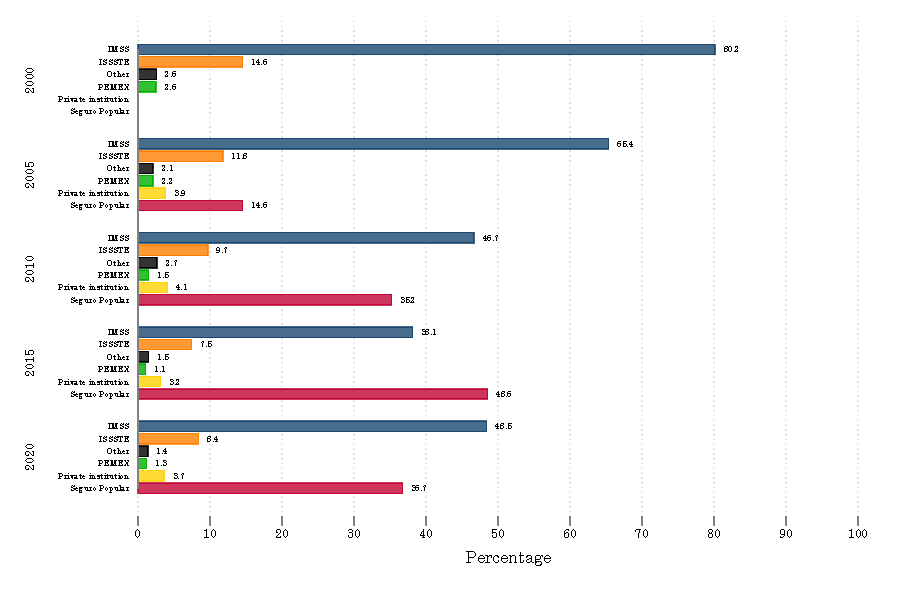
\includegraphics[width=\textwidth]{Figuras/derechohabiencia.pdf}
    \end{subfigure}
  \end{center}
  \scriptsize 
    Constructed with data from the 2000, 2010 and 2020 Censo de Población y Vivienda, the 2005 Conteo de Población y Vivienda and the 2015 Encuesta Intercensal, all conducted by INEGI. Each bar represents the proportion of people who claimed being insured by each institution. In particular the question they answered was \textit{Are you affiliated or do you have right to use the medical services provided by \texttt{institution name}?} Where \textit{\texttt{institution name}} is one of: IMSS, ISSSTE, PEMEX, Private institution, Seguro Popular, Other or None. For the year 2000 the answer option ``Private institution'' was not available.
    %\textit{Scripts: }  \texttt{insurance\_affiliation.do}
\end{figure}



\subsection{The Seguro Popular}

The Seguro Popular (SP) - formally known as the Sistema de Protección Social en Salud - was a Universal Health Coverage (UHC) scheme enacted by law in 2004 and targeted to the population not covered by social health insurance. SP was devised as a voluntary health insurance option which was made available to those not covered by IMSS or ISSSTE. A new financial architecture was implemented to promote more equitable health budget appropriations across all states.  Yearly health budgets to states were made in direct proportion to the number of families they managed to enroll and re-enroll year after year.   The SP financial scheme consisted of a tripartite arrangement, seeking to emulate the financing of social health insurance. The Federal government  contributed in equal terms to SP as it did to IMSS. The state governments used their own tax revenues to substitute for the employer's contribution. These funds were complemented by a means-tested premium paid by families. In practice, the three lower wealth deciles were exempt and small amounts were charged to all others. This matching funds scheme created incentives for state governments to affiliate as many beneficiaries as possible.  

In other words while IMSS medical care was financed mostly by payroll taxes, SP medical care was financed by general taxes. As highlighted by \cite{Levy_2008} this conditionality was thought to create incentives for working in the informal sector, for the reasons argued in the ``distortion-towards-informality'' (DTI) argument described in the introduction.\footnote{An oversimplified  way to look at this is that by being registered at IMSS workers and employers are forced to pay payroll tax. If workers do not value the benefits offered by IMSS to the extent of the tax, there are incentives to avoid it and work informally. To compound the problem, by starting to offer free services, SP makes an IMSS-affiliated job even less  attractive for workers and employers as it is not longer necessary to get health care}.

Fresh funds were used by states to increase the supply and quality of services to respond to the health needs and promote re-affiliation. In practice this meant that more resources would be devoted to locations with less coverage and consequently finance gaps and access gaps were slowly closed. Seguro Popular covered a basic package of primary health care and essential hospitalization services funded by the per-capita allocation. A concomitant fund for the protection against catastrophic spending provided targeted per-case reimbursement for high specialty care. Thus, universal health care through SP was a combined progression of population coverage, incrementally expanded services and improved financial protection. 

The SP became a natural experiment to test the DTI. SP was implemented gradually; payment and enrollment mechanisms were first tested with a pilot and starting in 2004 coverage expanded geographically across states that signed up and within states across municipalities based on health need, organizational capacity to deliver services, and local budget space.  This staggered rollout became an essential component of the empirical strategy to identify the negative effects of social protection programs like SP on formal employment. Figure \ref{sp_geo_coverage} presents the geographical expansion across municipalities. By 2011, 29 States had reported universal coverage, while the three remaining ones reported 83 percent coverage.


At the same time as the geographical expansion was taking place the number and types of procedures covered was increasing. While at the start it only covered 91 interventions, as of 2011 the health benefit package of SP (\textit{Catálogo Universal de Servicios de Salud, CAUSES}) covered 275 interventions. This expansion was also significant in terms of spending. \cite{Campos} explain that while IMSS expenditure declined from 1.7 to 1.5 per cent of GDP from 2003 to 2008, financing to health outside of IMSS increased -- basically a SP effect -- from 0.8 to 1.2 percent of GDP in the same period. The expenditure was concentrated in ``catastrophic health expenditure'', but it also devoted resources to preventive care. \cite{CIDE} estimate that household savings from SP can be substantial, with SP achieving a decline of close to 30 percent in catastrophic health expenditure for every peso spent by households.


\vspace{.1in}
\begin{figure}[H]
     \caption{Geographical coverage of SP by municipality}
    \label{sp_geo_coverage}
    \vspace{-.2in}
\begin{center}
\begin{subfigure}{0.65\textwidth}
        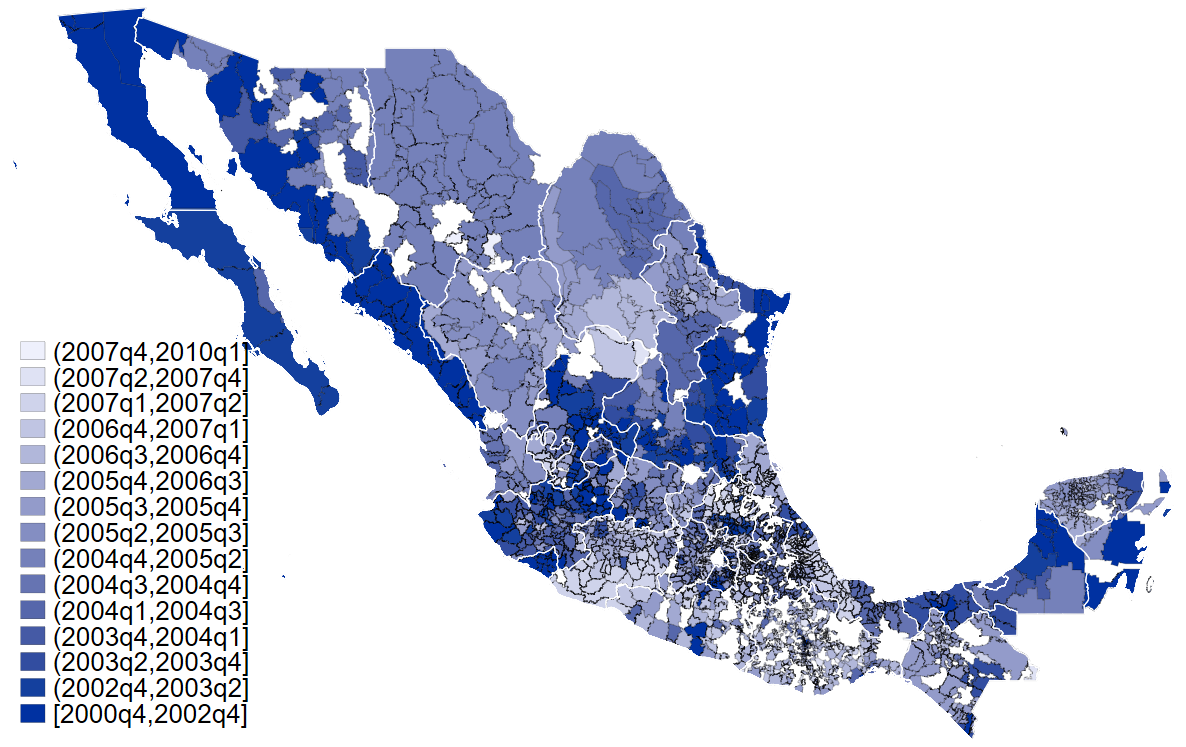
\includegraphics[width=\textwidth]{Figuras/sp_geo_coverage.png}
    \end{subfigure}
  \end{center}
    \scriptsize 
    \vspace{-.1in}
  This figure shows the geographic for SP. First municipalities to implement SP are shown in dark blue, while the last municipalities are shown in white. 
%\textit{Scripts: }  \texttt{sp\_geo\_coverage.do}
\end{figure}

\vspace{.1in}


SP helped close the gap in health expenditure between those registered at IMSS and ISSSTE and the rest. However as of 2010, public resources per beneficiary were still about 20 per cent higher in IMSS. Outpatient consultations 40 per cent higher and 2.6 times higher for specialty consultations. IMSS had also 30 per cent more nurses and 10 per cent more beds (Table 6 in \cite{Lancet}). Having less expense and inputs suggests also that SP provided more basic care than IMSS.

SP was legally repealed the 1st of January 2020 and replaced by the National Institute of Health for Welfare (or INSABI for its Spanish acronym).  The INSABI legal reform lacked details on how the financing transition from SP would take place.  Its implementation process to date has been highly disorganized and coincided with a Ministry of Health overwhelmed by the need to respond to the Covid 19 Pandemic.  Any formal assessment of the effects of INSABI on health coverage or labour market performance is still pending.  


\subsection{Formal jobs} 

This report will study the effect of SP on formal private sector jobs. This has several advantages. First, we know exactly when a job is registered at IMSS, thus allowing us to avoid measurement error in our estimate of private sector formal jobs - by definition. Second, we have full visibility of the job dynamics across the entire universe of formal salaried private sector instead of relying on samples as most papers using employment surveys (e.g. \cite{Azuara}) which cover less municipalities and are not representative at the municipality level. Actually, one might argue that the reason these papers have failed to find an effect on informality is precisely measurement error and small samples. Third, in our view the best published paper in the question of the labour market effects of SP uses this same data, and we have followed some of their methodological approach. This is also the only paper we know that has found a negative effect of SP on formal jobs. Using IMSS data allows us to test how robust this result is. The main disadvantage of using IMSS data is that we can only measure effects on private sector formal jobs. Not on public sector jobs, nor on informal jobs. 


\subsection{Some labour market statistics}

A cursory look at employment trends may give one clue of whether large changes in labour market are happening as SP was being rolled out. Figure \ref{informal_time} shows the unemployment rate, the labour force participation rate, and fraction of workers with IMSS from 2005 when ENOE started being collected to 2015. One can see that these three statistics are steady across these years, even though Seguro Popular coverage was growing strongly in these years.\footnote{From 2005 to 2015 SP incorporated close to 4 million extra beneficiaries.} One can also see that more than 70 percent of workers surveyed report not having IMSS coverage.   

\vspace{.2in}
\begin{figure}[H]
     \caption{Unemployment rate, labour force participation rate and fraction of workers without IMSS}
     \vspace{-.2in}
    \label{informal_time}
\begin{center}
\begin{subfigure}{0.55\textwidth}
        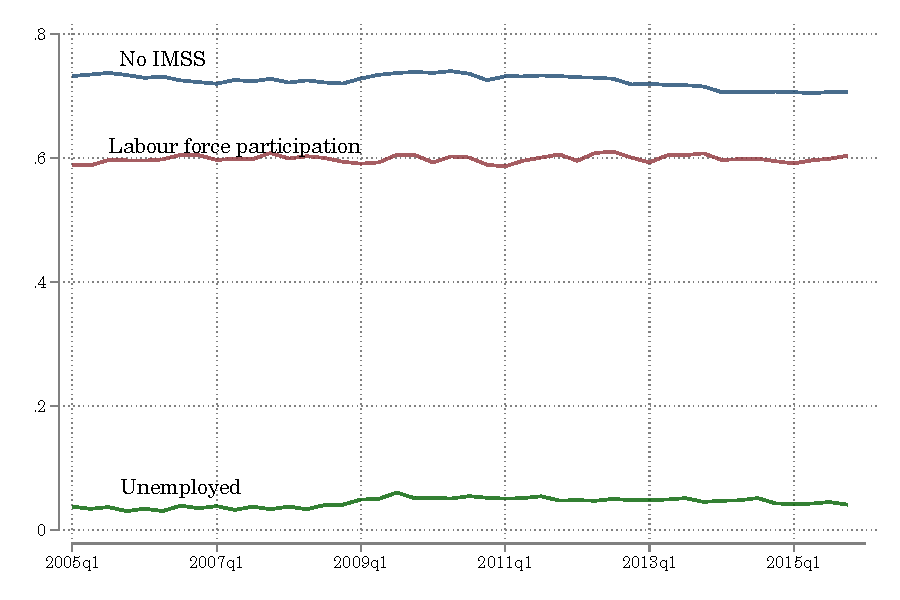
\includegraphics[width=\textwidth]{Figuras/unemp_noimss_labforce.pdf}
    \end{subfigure}
  \end{center}
    \scriptsize 
    This figure uses Mexico's employment survey ENOE from its inception in 2005 to 2015 to plot the unemployment rate defined as the proportion of people in the economically active population who \textit{do not} have a job (either formal or informal), labour force participation rate defined as the proportion of people older than 15 years who are either employed, unemployed or looking for a job, and the fraction of those employed that report not being registered with IMSS. ENOE covers 32 states encompassing 1584 municipalities between 2005 and 2015.
%\textit{Scripts: }  \texttt{informal\_time.do}
\end{figure}


%%%%%%%%%%%%%%%%%%%%%%%%%%%%%%%%%%%%%%%%%%%%%%%%%%%%%%%%%%%%%%%%%%%%%%%%%%%%%%%%%%%%%%%%

\section{Brief review of the literature} \label{literature}

As mentioned in the introduction, the question that frames the larger debate we are interested in, is whether social protection policies like health insurance or health care, income transfer programs, and others, generate inefficiencies and in particular engross the size of the informal sector at the expense of the more productive formal one. This is too large a question to be tackled in one paper. It is also an ill posed question as the details of the policy and its context should matter and have to be specified. We therefore focus on a narrower but important question having to do with Seguro Popular. The question this report is concerned with is whether SP decreases the number of formal sector jobs in the non-governmental sector. In the introduction we discussed why studying SP is important for the larger debate. This brief literature review aims only to discuss some of the most prominent papers studying this question, and the related question of whether SP increases the number of informal jobs. 

With the exception of \cite{Campos} every other paper we reviewed uses surveys to study the effect of SP. As we mentioned above this is problematic since other than the population census, Mexico does not have a survey that is representative at the municipality level for all its municipalities, and SP was implemented at the municipality level for all of them. Moreover, surveys are self-reported by workers and they may not know if they are enrolled in IMSS or not, as the employer is the one doing the registration. 

\paragraph{Using survey data.} One of the first papers on this issue is by \cite{Barros}. The paper uses several rounds of Mexico's Income-Expenditure survey together with the rollout of SP to measure effects on labour market outcomes. The paper finds no effect on labour force participation, hours worked, or relative wages of members of households already covered by IMSS versus those not covered. The later ones should be more affected by SP but the paper finds they are not. The author writes ``I find that SP did not induce a shift of workers into the informal sector''. He conjectures this is due to lower quality of care not being attractive to those with IMSS provided medical care. \cite{Knox} use employment surveys (which cover 33 cities) and finds ``little evidence of any correlation between Seguro Popular and the decision of workers to be employed in the formal or informal sector''. \cite{Azuara} is yet a third paper on this question. They use employment surveys and ``estimate that Seguro Popular had no effect on informality in the overall population''. Partitioning into sub-samples, they find an effect of 0.8 percentage point increase in informality for those with less than 9 years of education.\footnote{Partitioning in sub-samples without taking into account that they are estimating multiple hypothesis leads to the wrong standard errors however.} \cite{Pages} also use the employment survey. Using its short panel structure, they find that SP decreases the probability that a household is covered by IMSS by 0.3 percentage points on a base of 43 per cent.  All these papers show a zero or a negligible effect of SP on informality. 

\paragraph{Using administrative data.} The only paper we know of that uses administrative data is \cite{Campos}. The paper uses data from IMSS at the municipality level to compare the number of jobs and the number of formal employers\footnote{Firms registering at least one worker in IMSS.} in IMSS, across municipalities that had not yet implemented SP versus those that had already implemented it. They don't find any effect of SP on the number of formal jobs on average. But for firms of one to five employees, they find a decrease of 2 percent of formal jobs one year after implementation and in 4-5 percent four years after. They also find that one year after implementation the number of formal \textit{employers} decreased by 1.4 percent, and by 4.4 percent one and four years after, respectively. They estimate that this translates into a cumulative 2000-2011 loss of 36,000 employers and 171,000 employees from that would have formally registered with IMSS. On this we have three comments. To us this seems like a small number when compared for instance to 14 million workers registered in IMSS in 2010. The effect comes entirely from firms with less than five workers, which several authors have documented are the least productive. These firms may have similar productivity as firms in the informal sector, implying little change in aggregate productivity. But more importantly, we find that these results are not robust. They disappear once the analysis includes \textit{either} of the following: (1) all municipalities for which one can get data, (2) econometric methods which are robust to the effect of SP being different in different municipalities, (3) following workers individually and controlling for their time invariant characteristics, (d) other methodologies to estimate causal effects like instrumental variables, which rely on different identification assumptions. 

\vspace{.1in}
\noindent All in all we conclude there is not a single robust result in the literature showing that SP reduced formal jobs. If there are distortions from this social protection policy, they are not detectable on this margin.




%%%%%%%%%%%%%%%%%%%%%%%%%%%%%%%%%%%%%%%%%%%%%%%%%%%%%%%%%%%%%%%%%%%%%%%%%%%%%%

\section{Data} \label{data}

Before testing the three hypotheses we laid out, we start by describing the sources of data we use. Some of this data has not been put together before this report. 

\subsection{IMSS data}

Our main data source is IMSS. The law mandates that all private sector employees must be registered at IMSS and pay the corresponding contributions to IMSS. This entitles the workers and their families to a package of social security benefits including health care, life and workers compensation insurance for on the job injuries, old age and disability pensions and child care. The following are two sets of data provided by IMSS.

\paragraph{Municipality level data.} We were able to obtain data at the municipality level by quarter on the number of formal workers as registered in IMSS, and the number of firms registering formal workers, from the year 2000 to 2015. We observe the number of permanent workers and the number of temporary workers by gender and rural/urban areas. We also observe the average salary of those workers in the municipality. Additionally, we use the data published by \cite{Campos} in the AEA Policy webpage and complement it with our own. IMSS geographical affiliation and revenue collection structure does not exactly coincide with all municipalities, but most do. This means that we have data for close to 1700 municipalities. We will use this data to test hypothesis H1. This is the best data Mexico has to offer on formal private sector jobs. We were also able to obtain average wages for jobs registered with IMSS. This allows us to test hypothesis H3.

\paragraph{Individual level data.} We had access at IMSS premises to worker level data. The data set preserved anonymity of both employers and workers. Our sampling is as follows. We draw a simple random sample of 10 per cent of all workers that were enrolled in IMSS on January 2000. We then follow them across quarters from January 2000 to December 2019. This amounts to 52 million observations in total and allows us to inquire if the same individual left formal employment as a function of the introduction of SP. This data allows us to test hypothesis H2. It also allows us to test if the effects of SP differ by salary, type of worker, and labour histories. 


\subsection{Data from Seguro Popular}

We have data for the number of enrollees in SP by quarter from 2000 to 2009. This data was published by \cite{Campos} at \href{https://www.openicpsr.org/openicpsr/project/114886/version/V1/view}{OpenIPCSR}. It contains the number of beneficiaries enrolled in SP by municipality by quarter-year. We were also able to obtain a similar data but at the municipality-\textit{year} level directly from government publication at \href{http://datos.gob.mx/busca/dataset/beneficiarios-de-proteccion-social-en-salud-de-seguro-popular}{the open government data repository} for the full period when SP was active, from the years 2004 to 2019. We checked that these two datasets are consistent. The data allow us to define when a municipality implemented SP and thus track the roll-out of SP. We define a municipality as implementing SP when at least 10 people are enrolled in the municipality\footnote{Results are similar when we consider a threshold of 1 up to 100 beneficiaries when defining implementation of SP.} This data allows us to construct our main explanatory variable, which is whether and when a municipality implemented SP. It allow us to compare job outcomes for municipalities with and without SP at a given point in time.

\subsection{Data on clinics and hospitals.} We were able to obtain data indicating where  Mexico's hospitals and clinics are located, using GPS coordinates. The data includes the number of health facilities, the number of consulting rooms, and hospital beds. It also identifies the institution in charge of such health clinics. There are 32,393 primary care clinics, 5,081  hospitals, and 187 other health facilities (e.g. ambulatory specialty care or diagnostic and imaging health units). Figure \ref{map_clinics} in the Appendix maps the stock of medical infrastructure in Mexico. This data allows us to implement a new causal estimation method (``instrumental variables'') that uses the presence of clinics to generate earlier adoption of SP. Having different estimation methods is important to assess robustness of results since these methods rely on different assumptions.


\subsection{Data from the National Statistics and Geography Institute (INEGI)}

\paragraph{Employment surveys.} Mexico's INEGI experimented with a labour survey (first ENEU then ENE) in 2000-2004 and discontinued it as it seemed to have problems. It then started a new better quality survey called Encuesta Nacional de Ocupación y Empleo (ENOE) that has been running since 2005.  ENOE is a rotating panel, following the same person for 5 quarters maintaining an overlap of 80 per cent and rotating 20 per cent of the sample per quarter. It surveys on average about 312,000 people each quarter. We use data from the first quarter of 2005 to the last quarter of 2015. This implies we have 1.4 million individuals but just over 13 million observations. We define a person as working if they answered affirmatively to the following question: \textit{Did you work for at least one hour last week?}. And we consider it formal if they reported to be affiliated to IMSS. We use ENOE to study whether workers with IMSS have different observable characteristics, transition between the formal and the informal sector for the same person, and to estimate by how much their salary decreases when switching to the informal sector.

\paragraph{Population Censuses.} We use data from the population census on 2000, 2010 and 2020, together with intercensal data on 2005 and 2015. We use this data to extrapolate population on each quarter with a constant growth rate for each of the 5 years gaps. We add population as a control in all regression specifications. 

\subsection{Other data}

\paragraph{Lights from space.} It is possible that municipalities adopting SP before others do intrinsically have different economic conditions. One would like to isolate every other cause of employment changes like macroeconomic trends at the municipality level, and just focus on the effect of SP on the labor market. That is, we  want to avoid attributing to SP changes in formal employment that would be associated with changes in economic conditions unrelated to SP. To do this we needed a measure of economic activity that exists at the municipality level and that is measured at least at the yearly frequency. Luminosity has these two properties. It has been used as a proxy for economic activity in the economics literature (e.g. \cite{Micha}), and it exists at yearly frequencies for Mexican municipalities. It turns out after doing the analysis that controlling for luminosity makes no much difference in the estimated effects of SP. 






%%%%%%%%%%%%%%%%%%%%%%%%%%%%%%%%%%%%%%%%%%%%%%%%%%%%%%%%%%%%%%%%%%%%%%%%%%%%%%%%%%%%%%%%%%%%%
\newpage


\section{Empirical Methods} \label{Methods}

The challenge of measuring causal effects of an intervention is to find ways to estimate what would have happened without it. Absent a randomized experiment there are several quasi-experimental ways to try to estimate such a counterfactual. We discuss two methodologies we use below.

\subsection{Difference in Differences}

Difference in differences (DiD) is a method that can be applied in the context of a differentiated geographical roll-out of a program. This is the method that \cite{Campos} used. The methodology of difference-in-differences compares outcomes of municipalities that implemented the program against those that have not implemented yet. To identify a causal effect the context needs to satisfy a ``parallel trends'' assumption, that requires that early implementing municipalities would have had the same outcomes as late implementing municipalities if SP had not been implemented.\footnote{This assumption is inherently untestable as it involves a counterfactual, but having both sets of municipalities have similar employment trends before SP is a common check.}  

\vspace{.2in}
\begin{figure}[H]
     \caption{Roll-out of Seguro Popular (replication)}
     \vspace{-.2in}
    \label{tsline_emp}
\begin{center}
\begin{subfigure}{0.65\textwidth}
        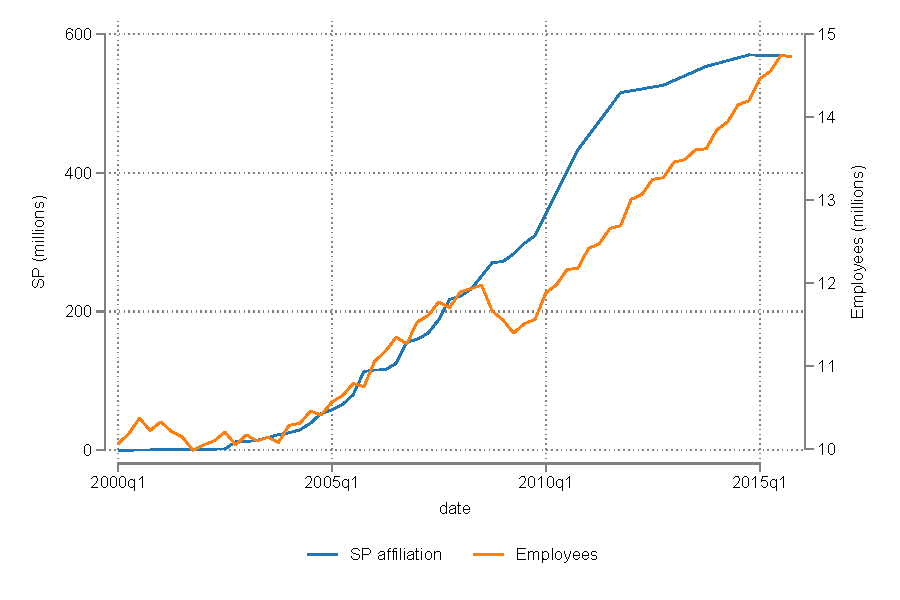
\includegraphics[width=\textwidth]{Figuras/tsline_emp_sp.pdf}
    \end{subfigure}
  \end{center}
  \vspace{-.15in}
    \scriptsize 
    SP refers to the number of beneficiaries enrolled in SP. Employees refers IMSS-registered employees. The numbers for SP and IMSS are individual level. SP registers all family members separately, while IMSS does not, that may explain the difference with Figure \ref{insurance_aff}. Information is quarterly.
    
%\textit{Scripts: }  \texttt{tsline\_emp.do}
\end{figure}


Figure \ref{sp_geo_coverage} already showed that the timing of adoption differed widely across municipalities. Figure \ref{tsline_emp}, shows the number of workers registered at IMSS (right hand vertical axis), and the individual affiliation to the SP program (left hand vertical axis).\footnote{Recall that IMSS registration entitles the entire family for medical care at IMSS, to to compare across the two lines one would have to multiply the IMSS numbers by family size. The numbers are similar if we assume IMSS beneficiaries have a family size of about 3.7.} As we have discussed above, it is a very large program in terms of the number of people covered. To the naked eye, it does not seem to be that there is much substitution across these two categories. The next section explores this more rigorously. The downturn of IMSS-registered jobs in 2008-2009 is associated with the worldwide financial crisis. 


\paragraph{Baseline model Specification.} We implement a DiD strategy by estimating a simple two-way fixed effect regression as follows:

\begin{equation} \label{DID_eqn}
  Y_{mt}=\sum_{k=-4}^{k=4}\beta_{k}\mathds{1}(\tau_{mt}=k)+\delta Pop_{mt} + \lambda_m + \lambda_t + q(t)\times s + \epsilon_{mt}
\end{equation}
 
\noindent $Y_{mt}$ denotes the log number of jobs registered at IMSS (or else the log number of employers registered) in municipality $m$ at time $t$. Time may represent a quarter-year or just a year.  $\tau_{m,}$ indicates the time before/after SP adoption, in particular $\tau_{mt}=0$ indicates the time of SP adoption. We will look at results four years prior and four years after implementation, therefore we have eight estimated coefficients: three for the pre-SP period ($\hat{\beta}_{-4}, \hat{\beta}_{-3}, \hat{\beta}_{-2}$)\footnote{We omit the coefficient $\hat{\beta}_{-1}$, so the rest of the coefficients are measured relative to the year before implementation.}. These allows us to test the assumption that formal job trends were parallel in earlier vs later implementing municipalities \textit{before} implementation.\footnote{Finding an ``effect'' of the program before program implementation ---that is finding that ($\hat{\beta}_{-4}, \hat{\beta}_{-3}, \hat{\beta}_{-2}$) are different from zero--- is a sign of mis-specification in the regression equation and would cast serious doubts on the appropriateness of the DiD method.} There is one coefficient for the year of implementation $\hat{\beta}_{0}$, and four coefficients for the years after implementation ($\hat{\beta}_{1}, \hat{\beta}_{2}, \hat{\beta}_{3}, \hat{\beta}_{4}$). Thus we are able to measure effects four years after. We control for the population of the municipality on logs $P_{mt}$, extrapolating linearly from the population census. We also control for a third-degree polynomial of time $q(t)$ interacted with state $s$ to allow for state-individual trends, and also by $X_{mt}$ which are municipality characteristics. Finally, we also include municipality ($\lambda_m$) and time fixed effects ($\lambda_t$). Two more details to note. Standard errors are clustered at the municipality level to take into account potential serial correlation in employment. We use weights that are proportional to the population in the municipality at year 2000. 



\vspace{.1in}
The regression specification in equation \ref{DID_eqn} is exactly the one used by \cite{Campos}. This allows us to assess the robustness of their results to three changes:

\begin{enumerate}
    \item Include time varying proxies for economic activity: in our case by including a third-degree polynomial of luminosity at the municipality-quarter level.
    \item Include more municipalities in the analysis. We were able to include 18 more municipalities that  \cite{Campos} dropped for lack of information on the number of enrollees in SP. We were able to obtain such data. Furthermore, we also use new data on employment we got from IMSS that enables us to include 300 municipalities more. At all times we use a balanced-panel of municipalities where we observe employment from 2000 to 2011, which spans 12 quarters before and 18 quarters after program implementation.
    \item Use a more flexible specification that allows earlier and later adopting municipalities to be on different time trends by interacting quarter of implementation interactions with time, as recommended by \cite{Wooldridge}.
    \item We use the methodology of \cite{deChaisemartin2020} which allows the dynamic effects of SP to be different in different municipalities. This may be the state of the art in terms of methods to implement a difference in differences design using the municipality rollout of SP.
\end{enumerate}


\paragraph{Flexible model specification.} What we call the ``flexible specification'' follows the advice of \cite{Wooldridge} and makes two additions to equation \ref{DID_eqn} above, represented in equation \ref{DID_eqn_flex} below:


\begin{equation} \label{DID_eqn_flex}
  Y_{mt}=\sum_{k=-4}^{k=4}\beta_{k}\mathds{1}(\tau_{mt}=k)+\delta Pop_{mt} + \lambda_m + \lambda_t + q(t)\times s +q(lum)_{m,t} + \gamma \mathds{1}(QI)_m \times t  + \epsilon_{mt}
\end{equation}

\noindent The additions are reflected in two terms: $q(lum)_m$ a third-degree polynomial of luminosity as proxy for economic activity, $\mathds{1}(QI)_m$ is an indicator variable for the quarter of implementation of municipality $m$ which we interact with a linear time trend $t$. These later interactions allow municipalities that implemented earlier to have different evolution of employment both before and after implementation than those that implemented later. There is no harm in including them: if municipalities turn out to have the same evolution of employment then the data will manifest that in that the $\gamma$'s will be statistically zero.  Rejecting that they are zero, however, means that the model in equation \ref{DID_eqn} is mis-specified, since it would be imposing a false assumption on the data, leading to biases in the estimates. We again cluster errors at the municipality level and use weights that are proportional to the population in the municipality
at year 2000.


\subsection{Individual level data and worker fixed effects}

We were able to obtain panel data on a random sample of 10 per cent of the workers who were at IMSS in January 2000. This enables us to follow particular workers and ask, for each of them, if they are more likely to terminate their IMSS-registered job when SP is implemented in their municipality. The ability to do this is important for several reasons. First, it enables us to study switching directly, and isolate gross flows out the formal sector from inflows which may mask the former at the municipality level. Second, it allows us to control for time invariant worker level characteristics, in the form of a worker fixed effect $\alpha_i$. The outcome variable is now an indicator for the worker $i$ living in municipality $m$ leaving IMSS at period $t$, $\mathbbm{1}(\text{worker leaves IMSS})_{imt}$. We cluster errors at the municipality level.

\begin{align} \label{eq_DID_individual}
  \mathbbm{1}(\text{worker leaves IMSS})_{imt}&=\alpha_i + \sum_{k=-4}^{k=4}\beta_{k}\mathds{1}(\tau_{mt}=k)+\delta Pop_{mt} + \lambda_m + \lambda_t + q(t)\times s \nonumber \\ 
  &\quad\quad\quad+q(lum)_{m,t} + \gamma \mathds{1}(QI)_m \times t  + \epsilon_{imt}
\end{align}


\subsection{Difference-in-Differences of dynamic effects}

Our preferred difference-in-differences method is that proposed by \cite{deChaisemartin2020}. We refer the readers to the original paper for detail. As they explain, this estimator is valid even if the treatment effect is heterogeneous across municipalities and across time. This estimation method resolves the problem of negative weights and bias generated by these. We implement this method using their STATA command \textit{did\_mutiplegt}.


\vspace{.1in}
\subsection{Instrumental variables}

The above methods use the staggered roll-out of SP to generate counterfactual outcomes; that is, outcomes that the implementing municipalities would have had if SP had not been implemented. This section implements a different empirical strategy; that of Instrumental Variables (IV). This method relies on a different identification assumption. It requires the existence of a variable (called an instrument) that can predict the implementation of the program at the municipality level (first stage), and that is by itself directly unrelated to the outcome we care about, which in this case is formal employment (the exclusion restriction). 

We have a candidate instrumental variable in our context. Because SP needed medical infrastructure to operate and not all municipalities had it, its implementation began in municipalities with enough clinics and hospitals. \cite{Campos} cite Mexico's Ministry of Health as stating that the geographies were chosen initially due ``to the capacity of offering the services, large concentration of urban and semi-urban population, and the existence of previous benefit programs from the government''. Based on this, we conjectured that the number of clinics and hospitals may predict which municipality implemented first and which implemented later, and therefore satisfy the statistical requirement of the first stage. Indeed we show later that this is the case. For the instrument to be valid however the number of hospitals and clinics does not directly impact the number of formal jobs in a municipality, once we control for population and other covariates. This is a strong assumption; it could be the case that municipalities with more hospitals per capita are richer or less healthy and that the number of clinics proxy for employment opportunities.\footnote{We provide some suggestive evidence of its plausibility. Figure \ref{trends_clinics} in the appendix splits municipalities by terciles of the number of clinics in the year 2000 and plots the evolution of formal employment.  It shows that that municipality with different medical infrastructure had similarly evolving employment trends before SP. Regression Table \ref{pretime_trends} tests this statistically.} 

\paragraph{First stage.} We first test if the medical infrastructure does indeed predict SP adoption at the municipality level. To do that we start with a set of potential instrumental variables given by the following list of variables: log(Total \# clinics), log(\# IMSS clinics), log(\# 2nd level clinics), log(\# 3rd level clinics), log(Total \# of rooms), log(Total \# of beds), Incumbency of political party. Using the above instruments, $Z_{mt}$, we estimate the following first stage equation that predicts the number of beneficiaries of SP at the municipality level $m$ for a particular quarter $t$:

\begin{equation} \label{first_stage_eqn}
    \log(\# \text{SP beneficiaries + 1})_{mt}= \alpha_0 + \beta'Z_{mt} + \nu_{mt}
\end{equation}

We then employ a Lasso method that selects which are the best predictors of implementation within the set of potential instruments. Lasso selected all but the  $\log$(Total \# of rooms) or  $\log$(Total \# of beds) for certain quarters, which we collectively call $Z_m$ and are measured in logs.

\noindent We estimate equation \ref{first_stage_eqn} separately for each quarter\footnote{The Lasso stage is also estimated separately for each quarter.}. We test if the coefficients in $\beta'$ are statistically different from zero using an F-test. Figure \ref{iv_fs} plots one estimated $\hat{Z}_m$ coefficient on the left Y-axis, they can be interpreted as elasticity. For instance, between 2006 and 2007, municipalities that had 100 per cent more clinics than others were between 90 and 150 per cent more likely to have implemented SP: a large correlation. The correlation is also statistically significant, with F-stats above 100 (right Y-axis), suggesting strong first stage instruments.


\paragraph{Second Stage.}  To estimate the effect of SP using our instrumental variable strategy we instrument the number of beneficiaries $\log(\# \text{SP beneficiaries + 1})_{mt}$ in equation \ref{IV_second_eqn} below using the first stage equation \ref{first_stage_eqn}.
\begin{equation} \label{IV_second_eqn}
    Y_{mt}=\beta \log(\# \text{SP beneficiaries + 1})_{mt}+\delta Pop_{mt} + \lambda_m + \lambda_t + (q(t)\times s) + q(lum)_{mt} + \epsilon_{mt}
\end{equation}

\noindent This equation is similar to the one we have been estimating, with the difference being that the independent variable that interests us is the number of SP beneficiaries in municipality $m$ at time $t$. The coefficient of interest is $\beta$, which can be interpreted as an elasticity: the percentage change in the number of jobs registered at IMSS over the percentage change in the number of SP beneficiaries. We would have full crowding out if $\beta=-1$. We instrument the number of SP beneficiaries in municipality $m$ at time $t$ with the predicted values from equation \ref{first_stage_eqn}, using two-stage least squares. We estimate equation \ref{IV_second_eqn} separately for each quarter and plot the elasticity through time in the main results on Figure \ref{iv_sp_dynamic} in the Appendix. 
Moreover, we also estimate equation \ref{IV_second_eqn} exploiting our panel data structure using a panel IV regression, and show results in Table \ref{paneliv_sp}.


\vspace{.2in}
\section{Main Results: Effects of Seguro Popular} \label{effects}

This section tests three of the hypotheses implied by the DTI hypothesis. Hypothesis 1 is that when SP is introduced in a municipality, workers switch from the formal sector (IMSS for the case of private sector formal workers) to the informal one. Implying that IMSS has less formal sector jobs registered at that municipality compared to municipalities that have (not yet) implemented. We cannot reject that there were no IMSS job losses. Hypothesis 2 posits that a given individual worker is more likely to abandon IMSS when SP gets introduced in his or her municipality. We cannot reject that there is no effect of SP on the probability of abandoning an IMSS-registered job. Hypothesis 3 focuses on the effect on wages. The DTI implies that the supply of workers to the formal sector decreases, as workers now offer their services in the informal sector. Without a change in the demand for workers in the formal sector, we would expect an increase in IMSS registered wages. We cannot reject that wages did not change as SP was introduced. We now present the results.

\subsection{Hypothesis 1: Effects on formal jobs}

\paragraph{Preferred specification.} Figure \ref{event_studies_emp} presents our main result, estimated in the \textit{exact sample and data} that \cite{Campos} use, but using the more robust econometric method of \cite{deChaisemartin2020}. Figure \ref{event_studies_emp} presents the result in graphical form, where the horizontal axis indicates the time periods in quarters. Zero indicates the quarter when SP was implemented in a municipality, negative numbers represent quarters before implementation and positive values quarters after implementation. The vertical axis measures the effect of SP on formal jobs in percentage terms. The shaded area represents 95 percent confidence intervals. If the shaded area crosses zero in the vertical axis, it means that we cannot reject the hypothesis of zero effect.

One would expect to find zero effects before the program is implemented. This is indeed what we find, lending credibility to the method. %Finding a different result would indicate that the parallel trends assumption was not holding before implementation and would cast doubt on the validity of estimating treatment effects using difference in differences methodology.
Figure \ref{event_studies_emp} - panel (a) shows the event for the number of firms registering workers at IMSS. Panel (c) shows the effect on the number of workers registered at IMSS. Finally, Figure Panel (b) focuses on workers in firms with only one employee, which we refer to as a ``self-employed'' worker. We focus on this sub sample. It is where \cite{Campos} found statistical effects in terms of employment. The main result is that we cannot reject the null hypothesis of zero effects. That is there is no evidence of SP decreasing either the number of firms registering workers, not on the number of registered workers themselves.

That our results are different from those of \cite{Campos} using their exact same data means that their estimate is likely biased and a result of the model not being robust to treatment effect heterogeneity. The new econometric literature summarized in \cite{DID_survey} shows that if early adopters benefit more or less from SP than late adopters, or are subject to different dynamics in treatment effects, then the specification used in \cite{Campos} gives biased estimates for the average treatment effect, indeed even the sign of the estimated effect could be wrong if the method implicitly uses negative weights. Indeed we find diagnostic indication that their methodology uses invalid negative weights. See Figure \ref{twfe_weights} in the Appendix. 



\begin{figure}[H]
     \caption{Event studies - Employment}
    \label{event_studies_emp}
\begin{center}
       \begin{subfigure}{0.4\textwidth}
    \caption{Employers at IMSS}
        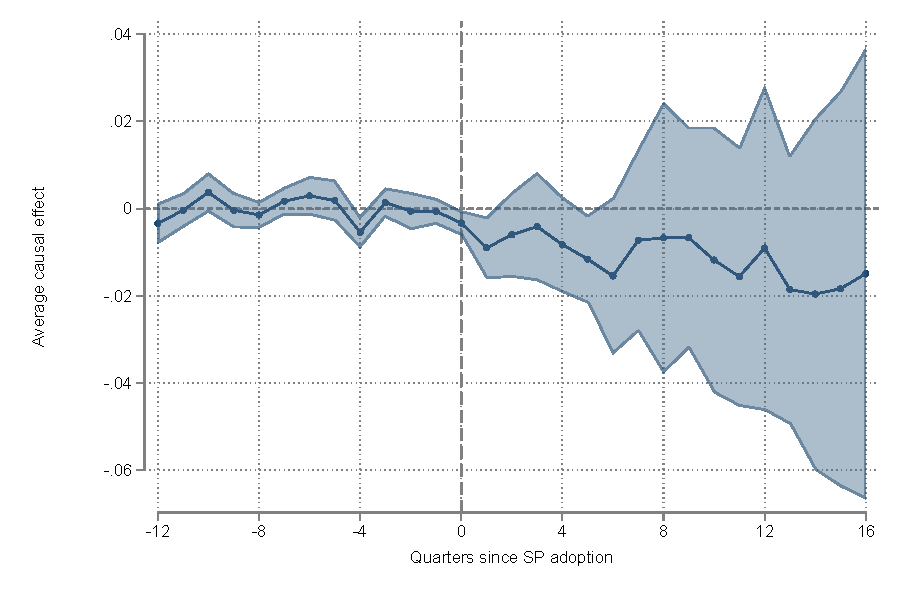
\includegraphics[width=\textwidth]{Figuras/did_event_ch_p_t.pdf}
    \end{subfigure}
    \begin{subfigure}{0.4\textwidth}
        \caption{Self-employed workers at IMSS}
        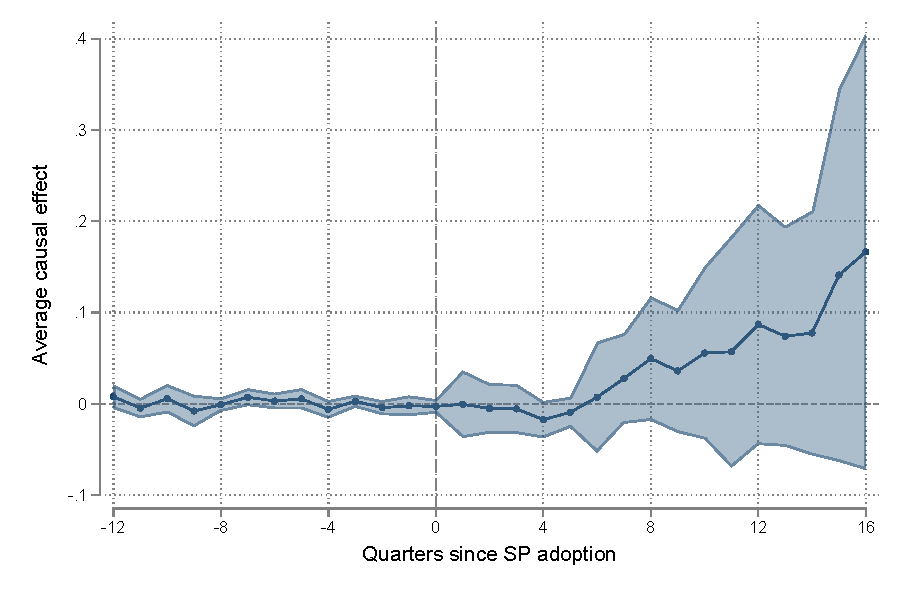
\includegraphics[width=\textwidth]{Figuras/did_event_ch_p_1.pdf}
    \end{subfigure}
        \begin{subfigure}{0.4\textwidth}
    \caption{Total IMSS workers}
        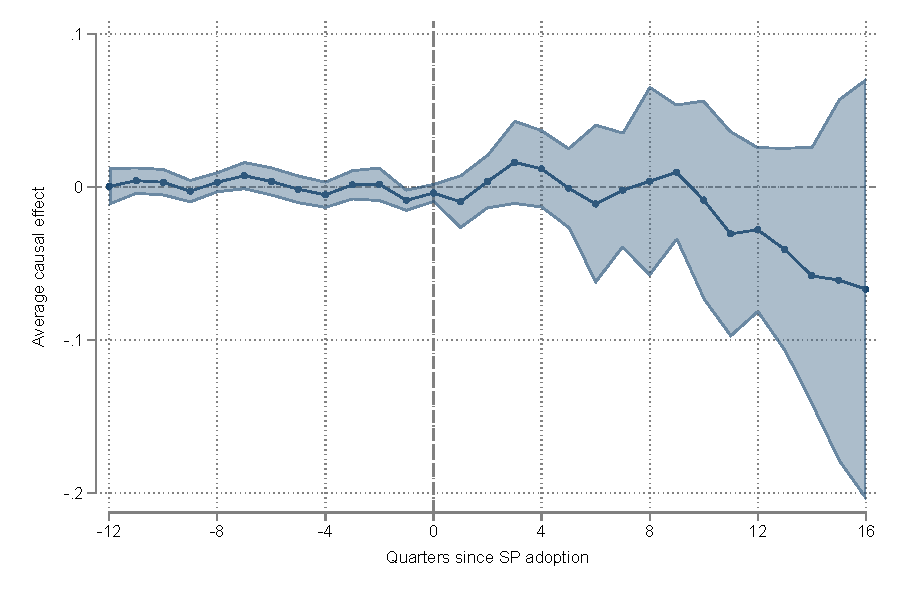
\includegraphics[width=\textwidth]{Figuras/did_event_ch_e_t.pdf}
    \end{subfigure}
  
  \end{center}
    \scriptsize 
    This figure plots the event studies for the introduction of SP and its impact in employment using our preferred specification the method of \cite{deChaisemartin2020}. Error are clustered at municipality level.
%\textit{Scripts: }  \texttt{did\_es.do}
\end{figure}



\paragraph{Replication of Bosch and Campos, 2014.} Given that \cite{Campos} is the only paper that finds negative effect of SP on formal jobs, we replicated their results using their data and their \textit{exact method} and found that it does replicate. Results of this replication are shown in Figures \ref{es_bc} in the Appendix.  We then assess the robustness of this result to 3 changes. 

\textit{Controlling for time-varying economic activity.} The first robustness check involves controlling for economic conditions at the municipality year level. Because Mexico's statistical agency does not produce GDP estimates at the municipality level, we use lights from space as a proxy for economic activity at the municipality level. The results survive almost unchanged (not shown). 

\textit{More municipalities.} A second robustness check is adding more municipalities to the sample. \cite{Campos} had to drop municipalities because information of the number of SP beneficiaries was missing for some or all periods considered in their analysis. We could recover 18 of them by accessing the SP census.\footnote{\url{https://datos.gob.mx/busca/dataset/beneficiarios-de-proteccion-social-en-salud-de-seguro-popular}.}  We could recover an extra 282 municipalities by complementing their data with new data at the municipality level from IMSS. We end up with 1692 municipalities compared to their 1,392.\footnote{Mexico has 2,454 municipalities, but 762 of them report zero workers to IMSS.} Figure \ref{es_more_mun} in the Appendix implements their exact estimation method to this larger sample of municipalities, so it evaluates the robustness of their sample using their own method. We find that the estimated negative effect for employers disappears. Moreover, that their methodology no longer delivers parallel trends before SP implementation for employees, and therefore does not afford a causal interpretation for employment results.

\textit{Flexible specification.} The final robustness check involves estimating the more flexible regression specification defined in equation \ref{DID_eqn_flex} on their exact sample of 1,392 municipalities. Figure in the Appendix \ref{es_flex} shows that their result is not robust to the more flexible specification.  The negative effects on IMSS-registered employers and on those single-employee firms disappears. Total IMSS-registered employees show a \textit{positive} trend, but it cannot be interpreted as causal because the trend is present before SP as well. The lack of robustness to including different time trends for municipalities according to when they implemented SP implies not a failure of their economic theory, but of their statistical model. Forcing municipalities to have the same evolution of employment imposes an assumption. We test and reject the assumption of homogeneous trends for earlier versus later adopters by testing that the $\gamma$ coefficients are zero in equation \ref{DID_eqn_flex}. We reject this null hypothesis for the case of employers and of workers with p-values of 0.0017 and 0.047, respectively. Imposing an assumption on the data that is false results in biased estimates.\footnote{Why do municipalities have different evolution of employment? This is a question lying outside the scope of the paper, but early implementing municipalities are larger as \cite{Campos} show, and they may be different in other respects, including industrial composition. These heterogeneity across municipalities makes it critical to allow for flexible estimation approaches \citep{Wooldridge}.}

\vspace{.1in}

The conclusion is then that the results of \cite{Campos} is nor robust. SP does not have an negative effect on average on the number of workers registered at IMSS (or on the number employers registering them). Below we explore if this conclusion holds not only on average, but also for particular sub-populations, and whether the method of instrumental variables delivers a different result. 


\subsubsection{Heterogeneity effect of SP}

This subsection asks if the effect of Seguro Popular significantly differs by gender, modality of IMSS employment\footnote{The data has 3 categories of IMSS affiliation: (1)  permanent workers -- those that have a labour relationship that for indeterminate time; (2) temporary workers -- those that have a labour relationship for a pre-specified task or time; (3) voluntary affiliates -- those that self-enroll in IMSS, presumably to have access to its services.}, workers in rural and urban areas, across the wage distribution of formal employees, and by marital status. For ease of interpretation, we split the sample in categories - in case of continuous variables defined by the median — and estimate our preferred specification separately for each category. In each case we also indicate with an orange dot if the estimates do not have parallel trends before SP implementation. This signals that we cannot trust these estimates as average causal effects.

\paragraph{Results.} Figure \ref{did_het} focuses on employees in all firms for 12 categories plotting the average effect through the 16 quarter post SP period. It finds null effects for all categories that have parallel trends. The negative coefficients for temporary and low wage workers cannot be trusted.   

\begin{figure}[H]
     \caption{Heterogeneous effects}
    \label{did_het}
\begin{center}
       \begin{subfigure}{0.55\textwidth}
        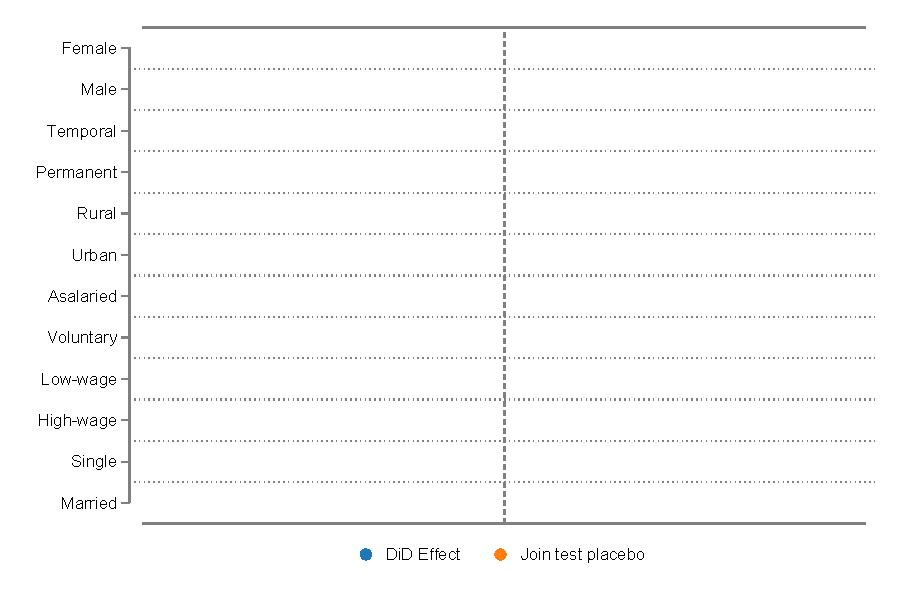
\includegraphics[width=\textwidth]{Figuras/did_het.pdf}
    \end{subfigure}
  \end{center}
    \scriptsize 
    
We plot the average dynamic effect for different categories. The command computes a weighted average of the $\text{DID}_t$ estimators, giving to each estimator a weight proportional to the number of switchers $\text{DID}_t$ applies to. Second, the command computes a weighted average of estimators similar to the $\text{DID}_t$, except that the outcome variable is replaced by the treatment.  This weighted average estimates the effect of first switches on the treatments that units receive after their first switch. Finally, the command computes the ratio of these two estimators. This ratio estimates the ``intention-to-treat'' effect of first switches on the outcome, and scales it by the ``first-stage'' effect of first switches on the treatments received thereafter. Accordingly, it estimates some average of the change in outcome created by a one-unit change in treatment.  Errors are clustered at municipality level.
%\textit{Scripts: }  \texttt{did_het.do}
\end{figure}



\subsubsection{Results using the Method of Instrumental Variables}

Table \ref{paneliv_sp} presents our instrumental variable estimates of the effect of Seguro Popular on the number of formal employers, the self-employed and the number of employees registered at IMSS. On average we find no effect on the number of IMSS-registered workers. we find that an elasticity of the number of SP enrollees on employers of -0.007, and on formal jobs of -0.003. This means that if the number of enrollees increases by 100 per cent then the number of jobs in IMSS decreases by 0.7, and 0.3 per cent, respectively. This is tiny. We find that all of the effect comes from firms with 1 employee (self-employment). Figure \ref{iv_sp_dynamic} in the appendix shows the IV results when estimating equation \ref{IV_second_eqn} separately for each quarter.


\vspace{.2in}
\begin{table}[H]
\caption{Effect of SP on Formal Jobs using IV strategy}
\label{paneliv_sp}
\begin{center}
\resizebox{0.55\textwidth}{!}{
\scriptsize{% Table generated by Excel2LaTeX from sheet 'paneliv_sp'
\begin{tabular}{lccc}
\toprule
      & \multicolumn{3}{c}{Employment} \\
\midrule
      & Employers & Self-employed & Employees \\
\midrule
      & (1)   & (2)   & (3) \\
\midrule
\midrule
Elasticity of SP & -0.0071* & -0.014* & -0.0031 \\
      & (0.0041) & (0.0081) & (0.0067) \\
      &       &       &  \\
\midrule
Observations & 30331 & 30331 & 30331 \\
Number of municipalities & 1626  & 1626  & 1626 \\
DepVarMean & 3.99  & 3.01  & 6.05 \\
Municipality FE & \checkmark & \checkmark & \checkmark \\
Economic activity controls & \checkmark & \checkmark & \checkmark \\
\bottomrule
\bottomrule
\end{tabular}%
}
}
\end{center}
 \scriptsize 
 This table presents instrumental variables panel regression estimates of the effect of SP on employers and employees registered at IMSS, as well as employers with 1 employee, which we call ``self-employed''. 
%\textit{Do file: } \texttt{iv\_sp.do}
\end{table}




\paragraph{Summary of the Test of Hypothesis 1.} Consistent with the overwhelming majority of the literature, we estimate that SP had no effect (or the effect is very close to zero) on the number of formal jobs, in our case measured as jobs registered at IMSS. 



%%%%%%%%%%%%%%%%%%%%%%%%%%%%%%%%%%%%%%
\vspace{.2in}
\subsection{Hypothesis 2: Effects on switching at the individual level} \label{HTE}

The second hypothesis \textbf{H2} tests whether workers already registered in IMSS in January 2000 are more likely to leave if SP is implemented in their municipality by estimating equation \ref{eq_DID_individual} by OLS, while including an individual level FE. For brevity, Figure \ref{es_ind} plots the average post-treatment effects instead of the complete time-profile of effects. We present results for the entire sample for close to 50 million individual-time observations (``All''), as well as further split the sample by (a) a measure of labour market attachment\footnote{Labour market attachment is measured as the percentage of time in a given period the person has not been enrolled at IMSS.}, (b) by whether the person had wages above or below the median in the year 2000 (``high wage'', ``low wage''), and (c) whether the worker worked on a single-worker firm (``self-employed''). Figure \ref{es_ind} finds tiny (almost null) effects on the probability of leaving an IMSS-registered job, with a \textit{negative} 0.2 percentage point increase. That is they are less likely to leave IMSS, but the magnitude is negligible.


\begin{figure}[H]
     \caption{Effect on the worker level probability of abandoning IMSS}
    \label{es_ind}
\begin{center}
       \begin{subfigure}{0.65\textwidth}
       %\caption{Flexible equation}
        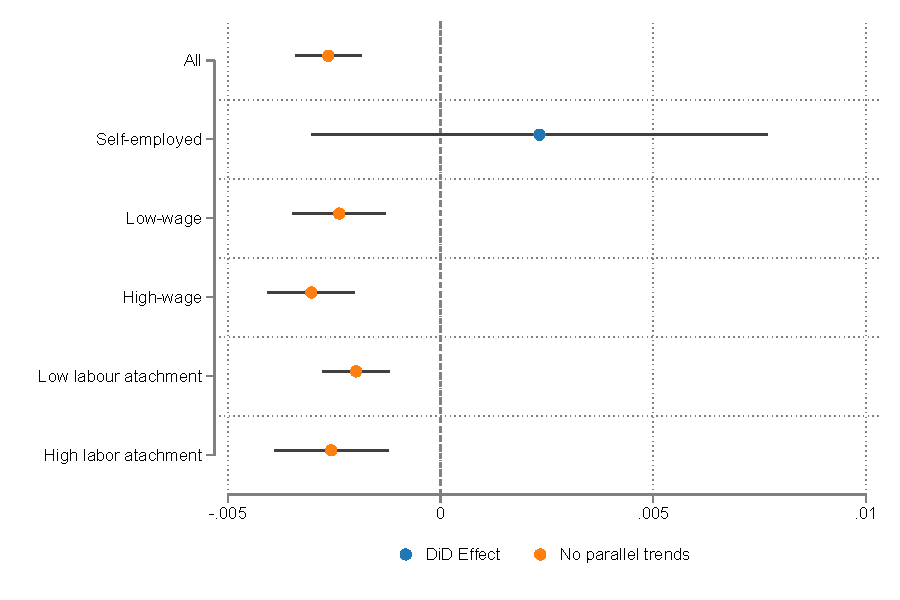
\includegraphics[width=\textwidth]{Figuras/did_imss.pdf}
    \end{subfigure}
     %  \begin{subfigure}{0.45\textwidth}
     %   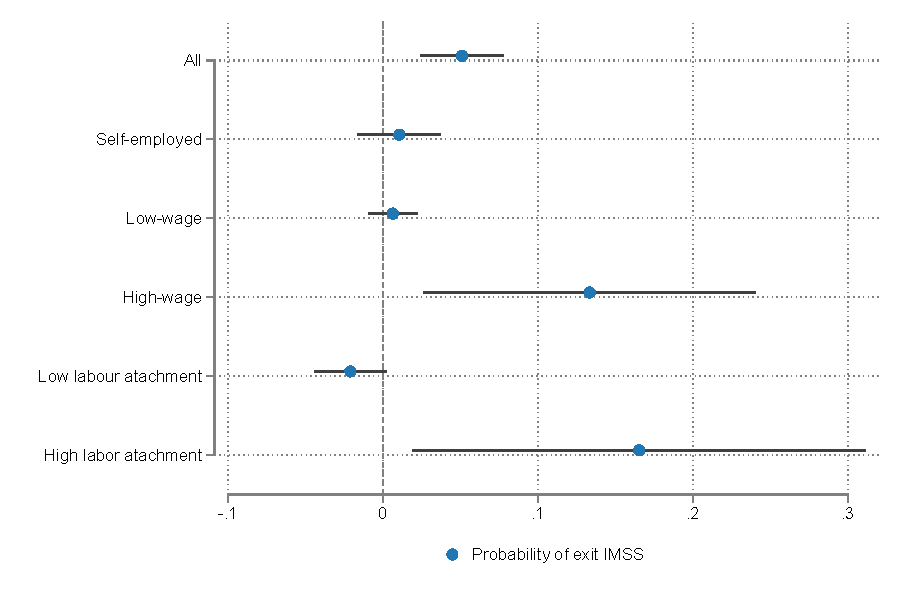
\includegraphics[width=\textwidth]{Figuras/did_ind.pdf}
    %\end{subfigure}
  \end{center}
    \scriptsize 
    
Effects of SP on probability of leaving IMSS estimating equation \ref{eq_DID_individual} using individual level data. %- Panel (a), and \cite{deChaisemartin2020} - Panel (b). 
We estimate equation \ref{eq_DID_individual} in all the sample (``All'') and also for different sub-samples. 
Standard errors are clustered at municipality level. Dots in orange fail the parallel trends tests.

%\textit{Scripts: }  \texttt{did_ind.do}
\end{figure}




\vspace{.2in}


\subsection{Hypothesis 3: Effects on average wages}

Given its significant size, if Seguro Popular has a disruptive effect in the labour market it could have the potential to change the salaries in the formal labour market. This could occur for instance if the supply of labour shifts from the formal and towards the informal market, given the benefits offered by SP only in the informal market. All else constant this would decrease equilibrium wages in the informal market and increase them in the formal one as formal employers try to compensate workers for not leaving.  Figure \ref{es_sal} estimates our preferred specification and plots the event study graph. As we can see, if anything we find a \textit{decrease} in wages, not an increase. But it is not statistically different from zero. 
%We also report the results using the IV methodology in Table \ref{paneliv_sp_wage}


\begin{figure}[H]
     \caption{Event studies - wages}
    \label{es_sal}
\begin{center}
       \begin{subfigure}{0.45\textwidth}
       \caption{Wages for total employees}
        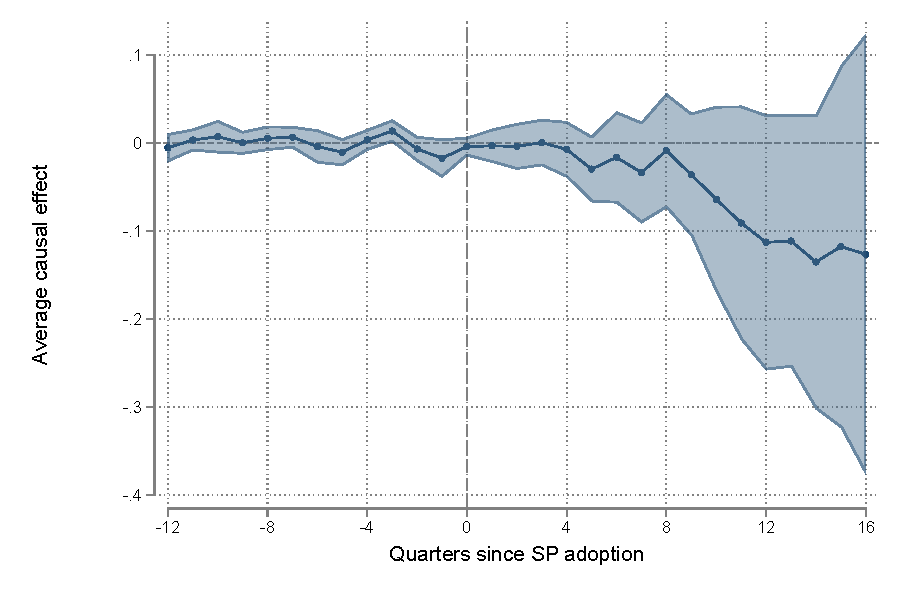
\includegraphics[width=\textwidth]{Figuras/did_event_ch_lg1_masa_sal_ta.pdf}
    \end{subfigure}
       \begin{subfigure}{0.45\textwidth}
       \caption{Wages for self-employed}
        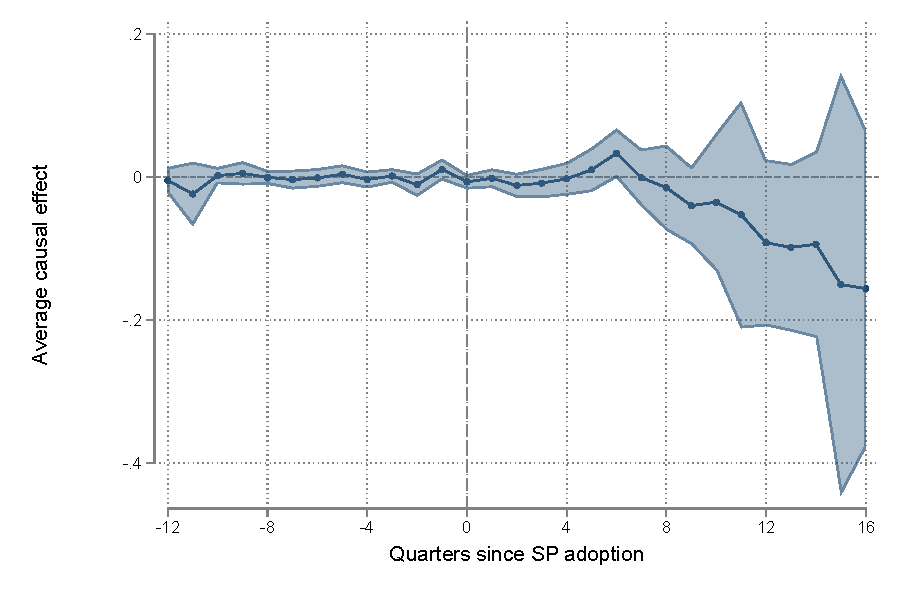
\includegraphics[width=\textwidth]{Figuras/did_event_ch_lg1_masa_sal_ta_1.pdf}
    \end{subfigure}
  \end{center}
    \scriptsize 
    
This figure plots the event studies for the introduction of SP and its impact in wages using our preferred specification the method of \cite{deChaisemartin2020}. Errors are clustered at municipality level.

%\textit{Scripts: }  \texttt{did_es.do}
\end{figure}


%\begin{table}[H]
%\caption{Effect of SP on wages using IV strategy}
%\label{paneliv_sp_wage}
%\begin{center}
%\resizebox{0.5\textwidth}{!}{
%\scriptsize{% Table generated by Excel2LaTeX from sheet 'paneliv_sp'
\begin{tabular}{lcc}
\toprule
      & \multicolumn{2}{c}{Wages} \\
\midrule
      & All   & Self-employed \\
\midrule
      & (1)   & (2) \\
\midrule
\midrule
Elasticity of SP & 0.022 & -0.016* \\
      & (0.019) & (0.0085) \\
      &       &  \\
Observations & 30714 & 30714 \\
Number of municipalities & 1642  & 1642 \\
DepVarMean & 5.61  & 4.04 \\
Municipality FE & \checkmark & \checkmark \\
Economic activity controls & \checkmark & \checkmark \\
\bottomrule
\bottomrule
\end{tabular}%
}
%}
%\end{center}
% \scriptsize 
%\textit{Do file: } \texttt{paneliv\_sp.do}
%\end{table}


%Table \ref{did_reg_sal} shows that we do not find an effect on formal worker salaries, but only a slight decrease in salaries on the self-employed of 1.4 per cent. We estimate the most flexible specification \ref{DID_eqn_flex}, while Table \ref{did_reg_sal_bc} in the Appendix estimates equation \ref{DID_eqn} using the municipalities that \cite{Campos} uses.

%\begin{table}[H]
%\caption{Difference in differences - salaries}
%\label{did_reg_sal}
%\begin{center}
%\resizebox{0.65\textwidth}{!}{
%\scriptsize{% Table generated by Excel2LaTeX from sheet 'did_reg_sal'
\begin{tabular}{lcccc}
\toprule
      & \multicolumn{4}{c}{Firm size} \\
\midrule
      & $=$ 1 & [2-50] & [51-250] & $>$ 250 \\
\midrule
      & (1)   & (2)   & (3)   & (4) \\
\midrule
\midrule
Four years prior & 0.028* & -0.026 & -0.061 & -0.21*** \\
      & (0.015) & (0.016) & (0.062) & (0.079) \\
Three years prior & 0.015 & -0.014 & -0.026 & -0.16** \\
      & (0.011) & (0.0093) & (0.044) & (0.061) \\
Two years prior & 0.0099 & -0.0011 & 0.0017 & -0.079** \\
      & (0.0065) & (0.0055) & (0.025) & (0.034) \\
      &       &       &       &  \\
Implementation & -0.014* & -0.0026 & 0.023 & 0.053 \\
      & (0.0076) & (0.0087) & (0.026) & (0.036) \\
One year after & -0.016 & 0.0037 & 0.048 & 0.14* \\
      & (0.011) & (0.012) & (0.042) & (0.073) \\
Two years after & -0.012 & 0.0038 & 0.081 & 0.25** \\
      & (0.015) & (0.014) & (0.058) & (0.11) \\
Three years after & -0.0044 & 0.0073 & 0.091 & 0.28* \\
      & (0.018) & (0.015) & (0.069) & (0.15) \\
Four years after & -0.0033 & -0.00025 & 0.100 & 0.30* \\
      & (0.021) & (0.017) & (0.079) & (0.17) \\
      &       &       &       &  \\
\midrule
Observations & 73944 & 73944 & 73944 & 73944 \\
Number of municipalities & 1699  & 1699  & 1699  & 1699 \\
R-sq  & 0.350 & 0.471 & 0.085 & 0.060 \\
DepVarMean & 3.97  & 4.90  & 3.65  & 2.39 \\
$H_0 : \alpha = 0$ (p-value) & 0     & 0     & 0.04  & 0.23 \\
\bottomrule
\bottomrule
\end{tabular}%
}
%}
%\end{center}
% \scriptsize 
%\textit{Do file: } \texttt{did\_reg.do}
%\end{table}





\section{Discussion} \label{discussion}

Given these results, one natural question to ask is why is SP \textit{not} causing a decrease in formal sector jobs nor an increase in formal sector salaries? The literature and this paper do not have a rigorous answer. This section puts forward some conjectures.

\paragraph{SP not valuable enough?} One possible reason is that SP not perceived as attractive enough to lure workers from the formal sector. SP does not cover all health treatments that medical care at IMSS covers; IMSS also has better infrastructure and anecdotally is perceived to provide higher medical care quality than SP. As of 2010, IMSS had about 20 per cent more public resources per beneficiary than SP. In terms of human resources and infrastructure, IMSS had about 30 per cent more nurses and 10 per cent more beds than SP.\footnote{These comparisons are imperfect because IMSS provides also child care and other services, although the overwhelming majority of spending is on health care.} If this is the case then lower quality can be acting as a screening device, attracting only workers with no access to IMSS while probing not tempting for IMSS workers. In addition, IMSS offers a bundled benefit package that is mandatory, incluing old age and disability pensions and childcare. Opting out of IMSS implies loosing out on all social protection coverages. 

\paragraph{Different industries and Different locations} One reason why IMSS workers may refuse to work in the formal sector is that they work in different industries and have acquired skills that are less useful in the informal sector.  Informality is concentrated on certain industries (see Figure \ref{informal_scian})\footnote{We are forced to use the classification IMSS data collects.}. Agriculture and livestock have more than 90 per cent of workers not affiliated to IMSS, followed by construction and several services. Informality is also very concentrated geographically, meaning the large shift from formal to informal jobs would mean either migrating to other municipalities, or deeply changing the economic structure of a given municipality, which may take time. 


\vspace{.05in}
\begin{figure}[H]
     \caption{Industrial and Geographical concentration of informality}
    \label{informal_scian}
\begin{center}
    \begin{subfigure}{0.50\textwidth}
    \caption{Industrial concentration of informality (ENOE data, 2005-2015)}
%\caption{ENOE (2005-2015)}
        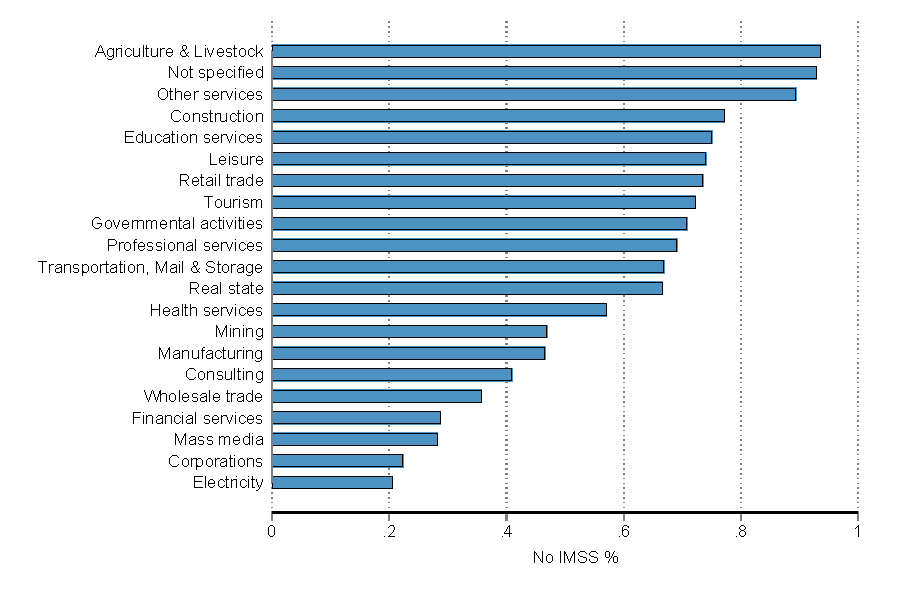
\includegraphics[width=\textwidth]{Figuras/catplot_scian_enoe.pdf}
    \end{subfigure}
    \begin{subfigure}{0.50\textwidth}
\caption{Geographical informality (2000, IMSS data)}
        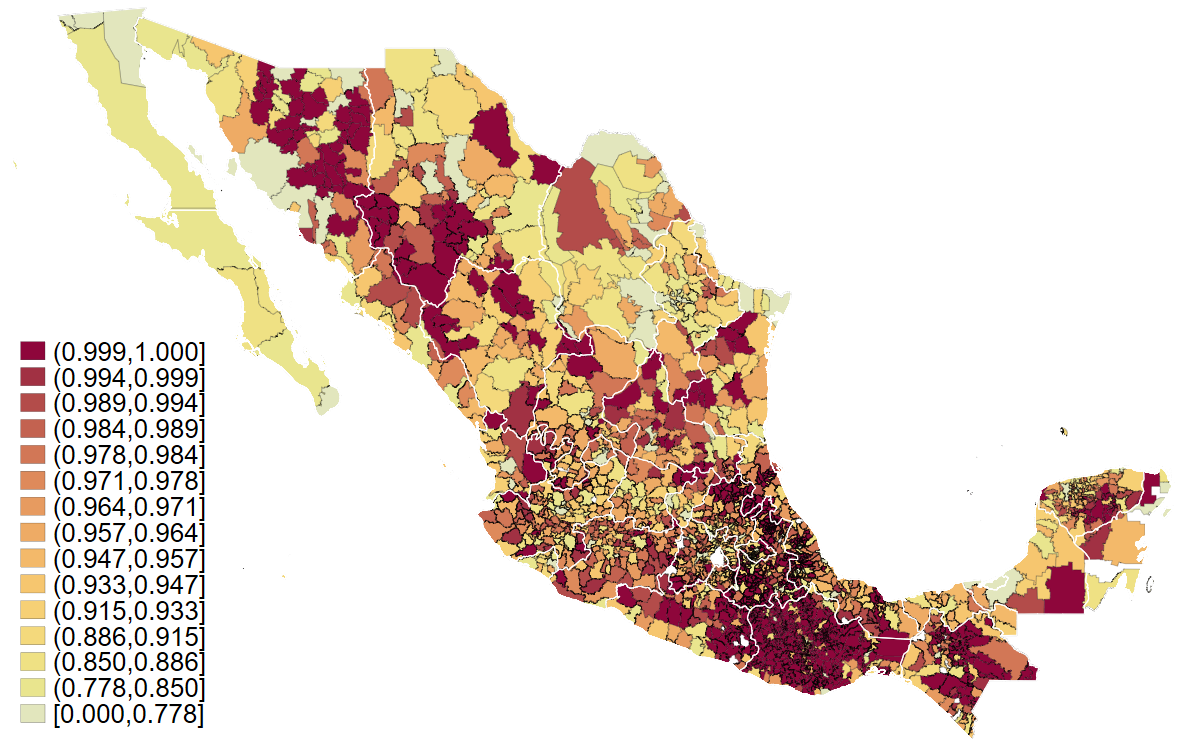
\includegraphics[width=\textwidth]{Figuras/spmap_porc_inf_2000.png}
    \end{subfigure}
  \end{center}
    \scriptsize 
    Panel (a) uses the ENOE survey (2005-2015) and plots the fraction of workers reporting that they are NOT affiliated to IMSS. Panel (b) is a map uses data from IMSS in 2000 to show the fraction of workers not covered by IMSS.  
%\textit{Scripts: }  \texttt{industrial_concentration.do, spmap_informality.do }
\end{figure}


\paragraph{Measuring flows into and out of informality.} One can try to measure flows into and out of formality. This faces an important problem: the only data that contains workers with and without IMSS for Mexico are the employment surveys. Their limitation is twofold: it only follows workers for five quarters, and whether they have IMSS or not is self reported and potentially subject to measurement error. Using the ENOE we calculate that the share of workers that switch from having an IMSS registered jobs to non-registered ones at some point in a 5-quarter span is 14.2 per cent.  Our concern is that it is just misreporting on the IMSS variable on the part of workers. Very often workers do not know whether they have or don't have IMSS.\footnote{In fact, IMSS has created an app called ``Reporte Personalizado de Cotizacion Individual'' precisely to inform workers if they are registered in IMSS or not as their employer is responsible for doing this procedure and often do not.} Even though some papers have argued using this data that flows are very prevalent across these two sectors, we believe these results are highly suspect because of measurement error. In fact, out of the of workers who are in IMSS in quarter one, only 2.9 per cent work without IMSS in quarter two and \textit{stay} there in quarters three, four and five. Moreover, 14.1 per cent of surveyed workers, make two or more switches between IMSS and NO-IMSS jobs in a span of five quarters. This seems too large to be believable.

\paragraph{Workers that report working informally and formally are different.}

We use the ENOE surveys to study if workers with versus without IMSS differ in their observed characteristics. To do this we estimate the following regression.

\begin{equation} \label{determinants_eqn}
    \mathds{1}(\text{no-IMSS})_{it} = \gamma_t + \delta_k + \alpha^\prime_m + \beta_j X_j + \epsilon_{it} 
\end{equation}

\noindent where $i$ indexes individuals surveyed in ENOE, $t$ indexed calendar quarter of the survey, $k$ indexes industries/occupations, and $m$ indexes municipalities, and $X_j$ are characteristics, indexed by $j$. We run a separate regression for each characteristic. It could be a dummy for being a woman, years of schooling, age in years, hourly wage (in logs), weekly hours worked, a dummy for holding two or more jobs, or a dummy for being married. We are interested in the coefficient $\beta_k$. We are controlling for quarter dummies ($\gamma_t$) that absorb macroeconomic trends in IMSS affiliation, this reduces spurious temporal correlations between IMSS affiliation and the business cycle for example. Some specifications also include municipality fixed effects ($\alpha^\prime_m$) and  industry fixed effects ($\delta_k$), which means that we are comparing characteristics of informal vs formal workers/jobs \textit{within} the same municipality and industry. 

Figure \ref{beta_characteristics_noimss} plots the estimated \{$\hat{\beta}_{j}$\} jointly for every characteristic. We statistically reject that coefficients are zero (confidence intervals are small enough to be subsumed in the dots). That is: informal and formal workers are different in their characteristics. This begins to cast doubt on models that assume that workers in both sectors are perfect substitutes. For instance, being a woman increases the likelihood of being informal by about 1.4 percent. An extra year of age increases the likelihood of informality by 4 percent. An increase of one sd in schooling (6.2 years) is associated with about 3 percent lower propensity of being informal. Analogously workers who work  one sd more weekly hours (18.7 hours) are about 7 percent less likely to be informal. It is likely that they differ even more in characteristics that would make them sort across formal/informal occupations, like occupation specific skills and experience, preference for flexibility in working hours, etc.


\vspace{.2in}
\begin{figure}[H]
     \caption{Characteristics and likelihood of not having IMSS coverage}
    \label{beta_characteristics_noimss}
\begin{center}
       \begin{subfigure}{0.55\textwidth}
        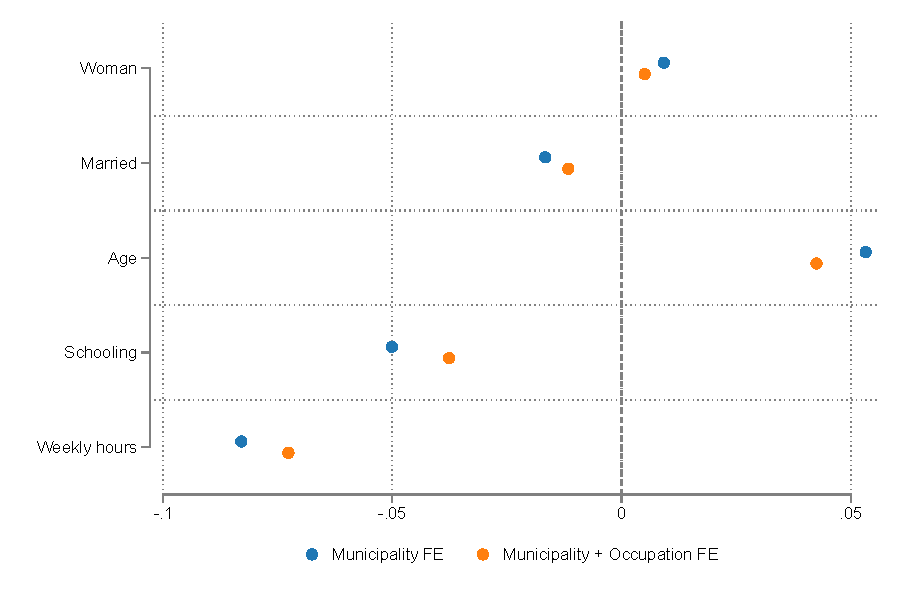
\includegraphics[width=\textwidth]{Figuras/beta_characteristics_noimss.pdf}
    \end{subfigure}
  \end{center}
    \scriptsize 
    This graph plots the estimates of $\beta_j$ using separate OLS estimated regression for equation \ref{determinants_eqn}. They measure correlation between not having IMSS and the displayed characteristic $X_j$.

%\textit{Scripts: }  \texttt{characteristics_informal.do}
\end{figure}


%To try to isolate differences between formal and informal workers we have controlled for municipality and occupation fixed effects. Do they matter? It turns out that municipality dummies explain alone 13\% of variation in not having IMSS, while occupation dummies alone explain 16\%. In contrast, demographics alone (gender, age, and years of schooling) explain only 4\% of variation. This means that, to an important extent, workers' variation in formality is determined geographically and also that they are concentrated on a subset of occupations. 


\paragraph{Salary changes.} Another reason formal workers may not quit their IMSS job and work in the informal sector after SP is implemented is that they may command higher salaries in the formal sector. For those that do switch, we estimate the following regression equation: 
\begin{align} 
    \log(\text{wage}_{it}) =&  \theta_i + (\gamma_t\times\alpha^\prime_m)  + \delta_k  + \beta\mathds{1}(\text{No-IMSS})_{it}+ \epsilon_{it}
\end{align}

\noindent where $i$ indexes individuals surveyed in ENOE, $t$ indexed calendar quarter, $m$ indexes municipalities, and $k$ indexes industries. Importantly we include individual fixed effects $\theta_i$. This means we are comparing the same person in two different kinds of jobs, formal and informal. We are interested in the coefficient $\beta$ which measures how big is the difference of a given person's wage in the informal sector.

We find that the salary earned \textit{by the same worker} is lower by 8 per cent in jobs not registered in IMSS (see Table \ref{salary_changes} in the Appendix). Since we cannot know whether they were fired or they themselves chose the informal job we cannot tell whether 8 per cent is a compensating differential unfortunately. This number is just meant to illustrate that informal jobs seem to carry lower salaries. If the ``No-IMSS'' variable was measured with (classical) error, the true difference may be even larger. This suggests that SP should command substantial value for workers to choose the informal sector over an IMSS job. 




%%%%%%%%%%%%%%%%%%%%%%%%%%%%%%%%%%%%%%





\section{Conclusion} \label{conclusion}

This paper evaluates the effect of Seguro Popular on the number of formal jobs and wages. We find first that SP did not decrease the number of formal jobs at the municipality level (H1) nor did it cause private sector workers employed in the private sector to quit the private sector job. We find no evidence of a more restricted supply of workers to the formal sector, in terms of equilibrium wages, as wages in the formal sector did not increase. This report uses more and higher quality data than existing studies, but reaches the same conclusion as most of the existing papers. The only exception to that conclusion was \cite{Campos}, but we find that their results are not robust, and are highly dependent to the municipalities selected, the regression specification used, and the identification strategy implemented. Changes in any of these items makes their result disappear. The most solid conclusion with the best available data and more robust methods is that SP did not decrease formal sector jobs in Mexico.  This does not mean that Seguro Popular had the best design available; indeed it is possible that universal health care that is not conditional on working in the informal sector could be better than SP. It only means that the quantity of jobs in the formal sector did not suffer as a result of its implementation.

In the introduction we noted that to rationally decide if a social protection program should or should not be implemented one has to look at both the cost and the benefit sides. Most of the literature of SP has looked at the costs, but in the light of evidence from health insurance in the US, the benefits could be large and important. The next step in evaluating Seguro Popular should be measuring its benefits, and more particularly the effects on financial protection and health outcomes. After all, this was the rationale for implementing it.
\newpage


%%%%%%%%%%%%%%%%%%%%%%%%%%%%%%%%%%%%%%%%%%%%%%%%%%%%%%%%%%%%%
%BIBLIOGRAPHY


\clearpage
\bibliographystyle{authordate1}
%\bibliographystyle{amsalpha}
%\bibliographystyle{AER}

\bibliography{References}

\nocite{GonzalezPier, GonzalezBarraza, Knaul}



%\FloatBarrier
%%%%%%%%%%%%%%%%%%%%%%%%%%%%%%%%%%%%%%%%

\newpage
\singlespacing


    
%__________________________________________________________________________
%__________________________________________________________________________



\newpage

% APPENDIX 
\setcounter{table}{0}
\setcounter{figure}{0}
\setcounter{section}{0}
\pagenumbering{gobble}

\begin{center}
	\LARGE Does Seguro Popular Reduce Formal Jobs?  \\[0.5em]
	\Large{Appendix $-$ For Online Publication} \\[1em]
	\large \author{Enrique Seira  \and Isaac Meza  \and Eduardo González-Pier \and Eduardo Alcaraz}
\end{center}

\appendix
\pagenumbering{arabic}
\renewcommand\thefigure{OA-\arabic{figure}}
\renewcommand\thetable{OA-\arabic{table}}
\renewcommand*{\thepage}{OA - \arabic{page}}
\renewcommand\thesection{Appendix \Alph{section}.}
\renewcommand\thesubsection{\Alph{section}.\arabic{subsection}}

%\renewcommand{\cftparskip}{0em} % NOT NEEDED
\renewcommand\cftsecdotsep{\cftdotsep}
\renewcommand\cftsubsecdotsep{\cftnodots}
\renewcommand{\cftsecnumwidth}{6em}
 \renewcommand{\cftpnumalign}{r}
%\renewcommand{\cftsecleader}{\normalfont\cftdotfill{\cftsecdotsep}}


\renewcommand{\cftsecleader}{\cftdotfill{\cftsecdotsep}\hspace{1.8em}}
%\renewcommand{\cftsecpagefont}{20em}
%\renewcommand{\cftfignumwidth}{6em}
%\renewcommand{\cfttabnumwidth}{3.3em}

%\tableofcontents
\etocdepthtag.toc{mtappendix}
\etocsettagdepth{mtchapter}{none}
\etocsettagdepth{mtappendix}{subsection}

\setstretch{0.9}
%\renewcommand\contentsname{} % the empty name

\begingroup
\let\clearpage\relax
%\vspace{-1.5em} % the removed space. Set as appropriate
\tableofcontents
\endgroup


\newpage

\vspace{.2in}

\section{Additional Results}


\begin{figure}[H]
    \caption{Health expenditure as proportion of current income}
    \label{health_expenditure_share}
\begin{center}
\begin{subfigure}{0.60\textwidth}
        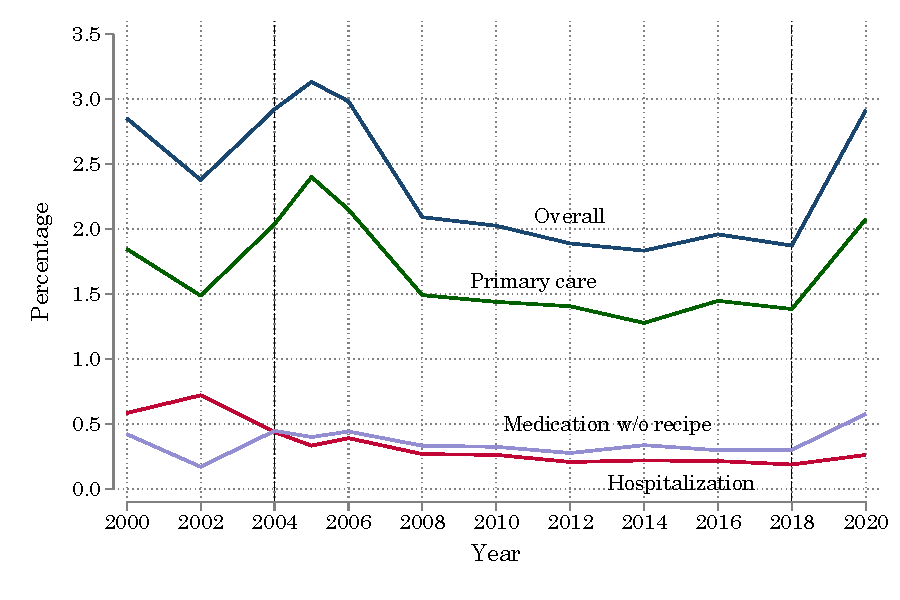
\includegraphics[width=\textwidth]{Figuras/oop_evolution_percentages.pdf}
    \end{subfigure}
 \end{center}
 \scriptsize 
    Vertical dashed lines denote beginning and ending of 
 SP program. This figure uses Mexico´s income and expenditure survey ENIGH - conducted by INEGI - from 2000 to 2020 to plot the mean health expenditure as proportion of a household's current income. To construct each variable we take the quarterly reported expenditure on each of the expenditure categories and make them annual quantities multiplying them by 4, as suggested by INEGI. We then standardize expenditure to 2018 Mexican pesos to make quantities comparable over time. Lastly, we divide each category's expenditure by the annualized current income to compute health expenditures as proportions of current income. For computing the mean we use frequency weights provided by INEGI in each survey. ENIGH data is collected every two years; in 2005 an additional survey was run in response to the demand for data by policymakers and researchers.
    %\scriptsize \textit{Scripts: }  \texttt{12_pocket_expenditure.do + aux_oop_graph.do}
\end{figure}

\vspace{.2in}



\subsection{TWFE diagnostics}
\begin{figure}[H]
     \caption{TWFE weights}
    \label{twfe_weights}
\begin{center}
       \begin{subfigure}{0.45\textwidth}
        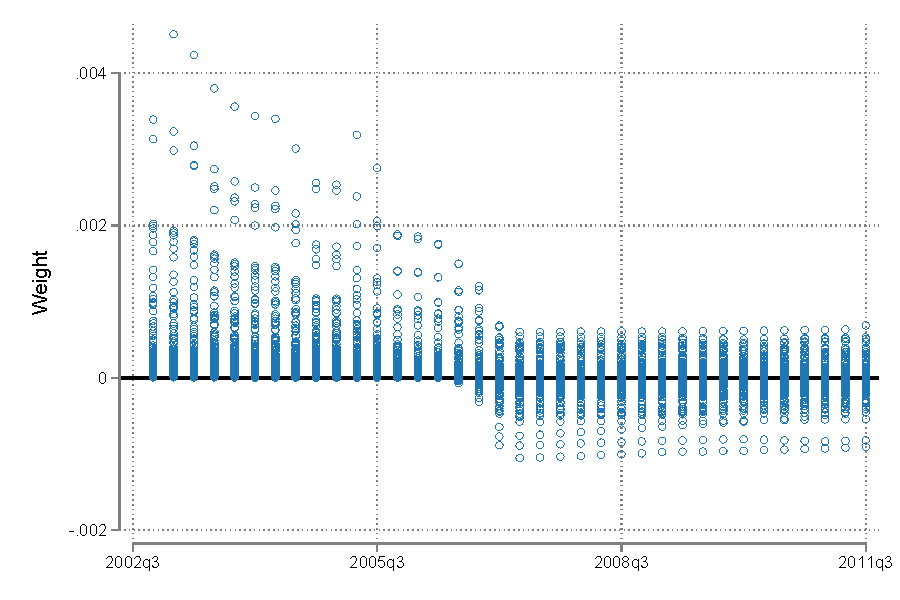
\includegraphics[width=\textwidth]{Figuras/twfe_w_p_t.pdf}
    \end{subfigure}
  \end{center}
    \scriptsize 
We compute the weights attached to the two-way fixed effects regressions studied in \cite{deChaisemartin_twfe_weight}, and using their STATA command - \textit{twowayfeweights}. Under the common trends assumption, beta estimates a weighted sum of 36741 ATTs. 26018 ATTs receive a positive weight, and 10723 receive a negative weight.
The sum of the positive weights is equal to 1.37.
The sum of the negative weights is equal to -0.37.
Observe that for the later quarters we find negative weights, so that the DiD estimates become biased for estimates 3-5 years after implementation. Exactly when \cite{Campos} find their larger effects.
%\textit{Scripts: }  \texttt{weights_twfe_diagnostic.do}
\end{figure}


\subsection{Replication \cite{Campos}}

\begin{figure}[H]
     \caption{Event studies - \cite{Campos} replication}
    \label{es_bc}
\begin{center}
       \begin{subfigure}{0.325\textwidth}
    \caption{Employers}
        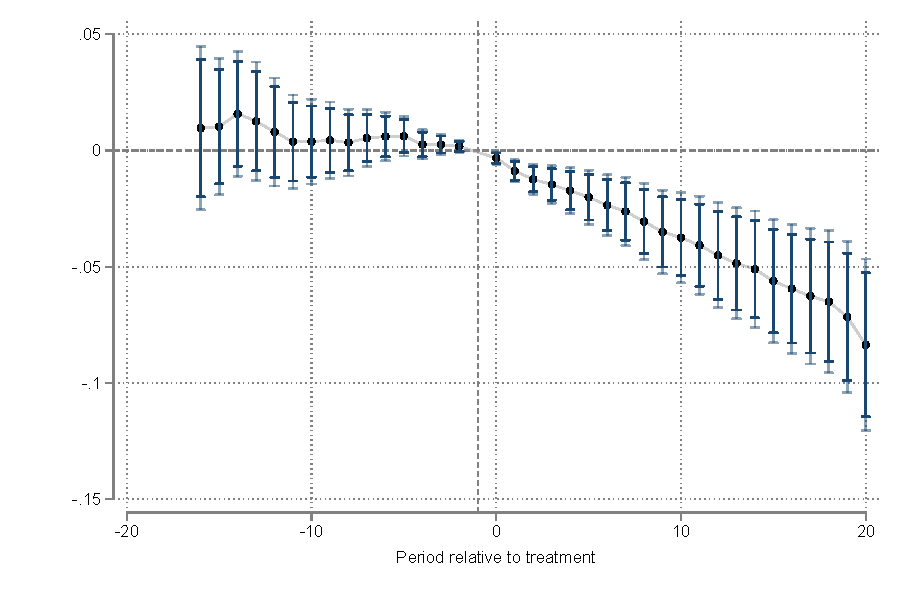
\includegraphics[width=\textwidth]{Figuras/did_event_bc_p_t.pdf}
    \end{subfigure}
    \begin{subfigure}{0.325\textwidth}
        \caption{Self-employed}
        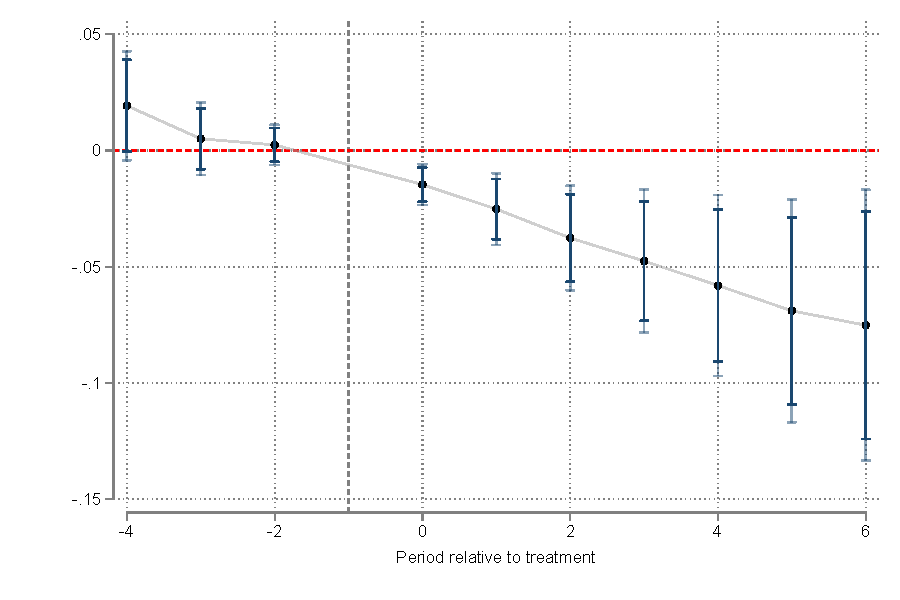
\includegraphics[width=\textwidth]{Figuras/did_event_bc_p_1.pdf}
    \end{subfigure}
        \begin{subfigure}{0.325\textwidth}
    \caption{Employees}
        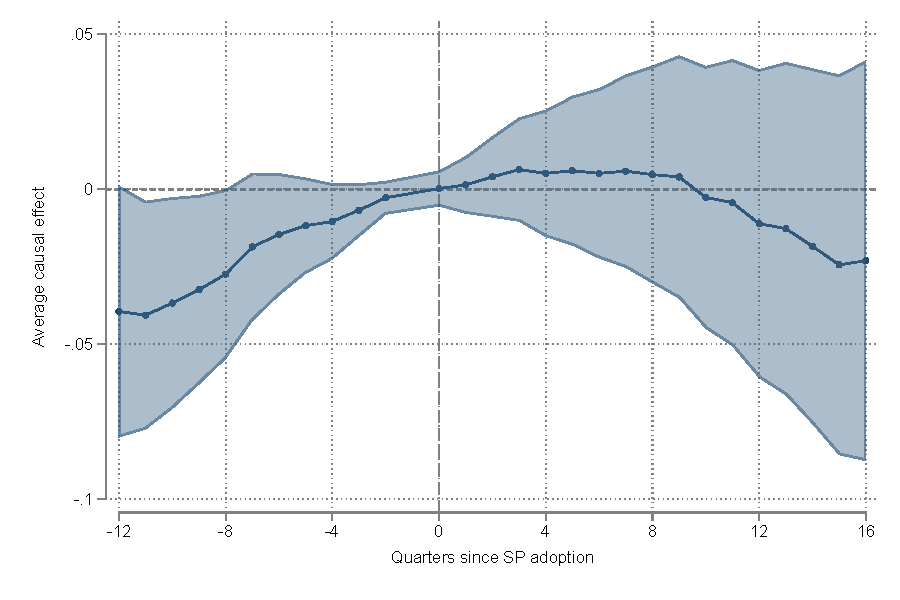
\includegraphics[width=\textwidth]{Figuras/did_event_bc_e_t.pdf}
    \end{subfigure}
  
  \end{center}
    \scriptsize 

%\textit{Scripts: }  \texttt{did\_bc.do}
\end{figure}


\subsection{Robustness analysis of \cite{Campos} specification}


\begin{figure}[H]
     \caption{More municipalities}
    \label{es_more_mun}
\begin{center}
       \begin{subfigure}{0.325\textwidth}
    \caption{Employers}
        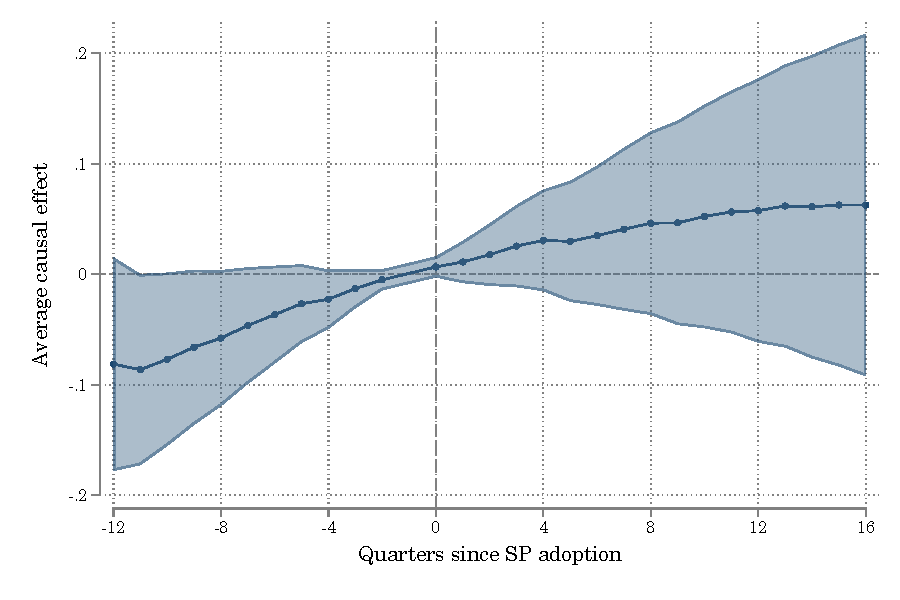
\includegraphics[width=\textwidth]{Figuras/did_event_mun_p_t.pdf}
    \end{subfigure}
    \begin{subfigure}{0.325\textwidth}
        \caption{Self-employed}
        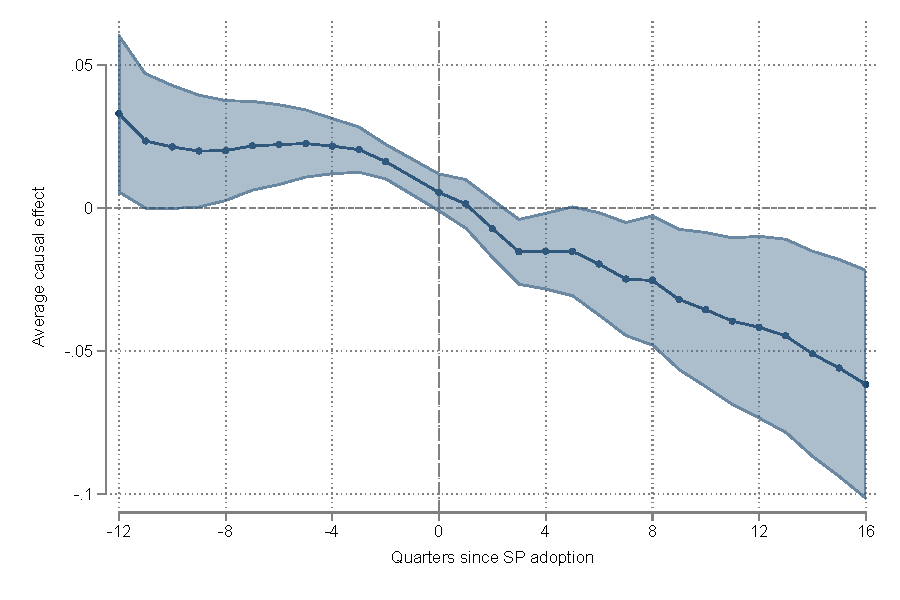
\includegraphics[width=\textwidth]{Figuras/did_event_mun_p_1.pdf}
    \end{subfigure}
        \begin{subfigure}{0.325\textwidth}
    \caption{Employees}
        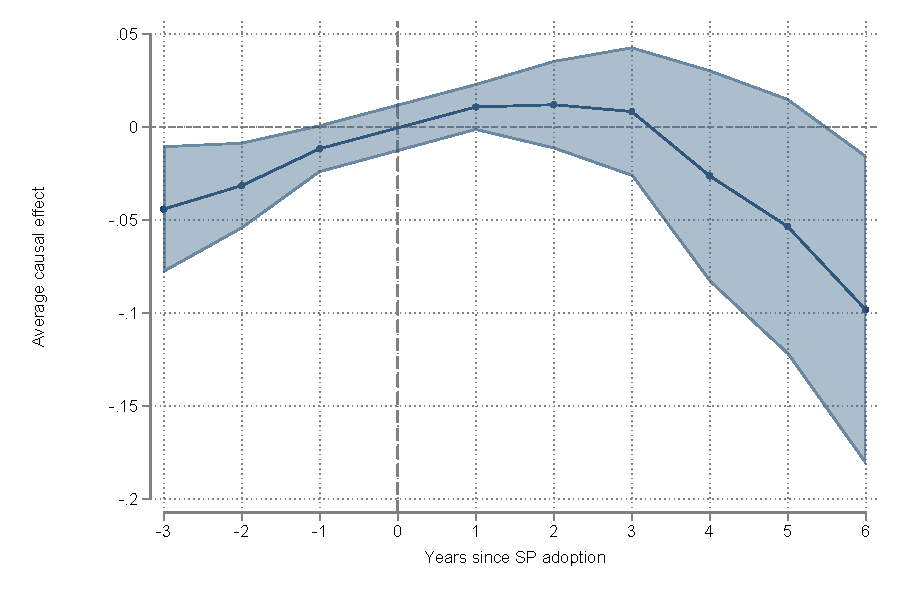
\includegraphics[width=\textwidth]{Figuras/did_event_mun_e_t.pdf}
    \end{subfigure}
  
  \end{center}
    \scriptsize 
%\textit{Scripts: }  \texttt{did\_es.do}
\end{figure}


\begin{figure}[H]
     \caption{Flexible specification}
    \label{es_flex}
\begin{center}
       \begin{subfigure}{0.325\textwidth}
    \caption{Employers}
        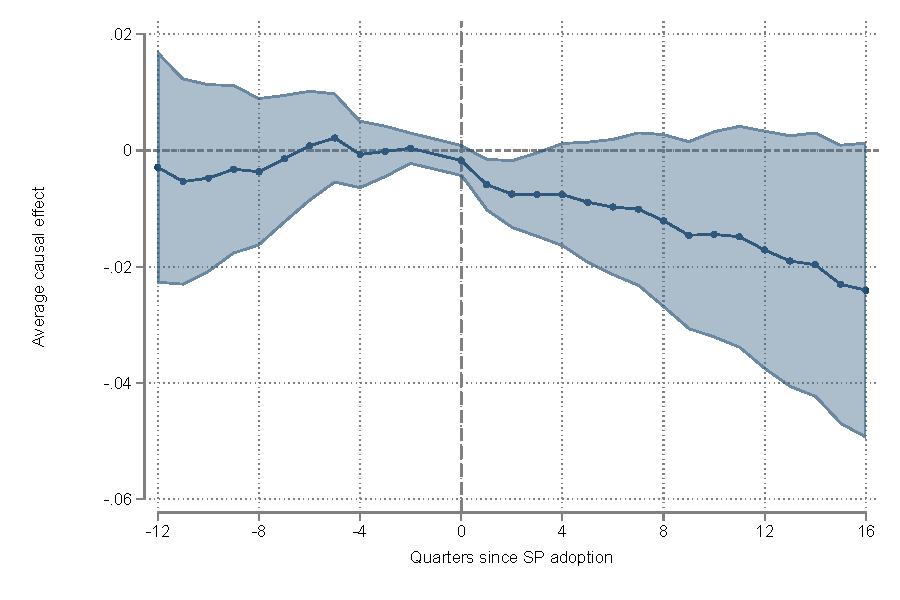
\includegraphics[width=\textwidth]{Figuras/did_event_flex_p_t.pdf}
    \end{subfigure}
    \begin{subfigure}{0.325\textwidth}
        \caption{Self-employed}
        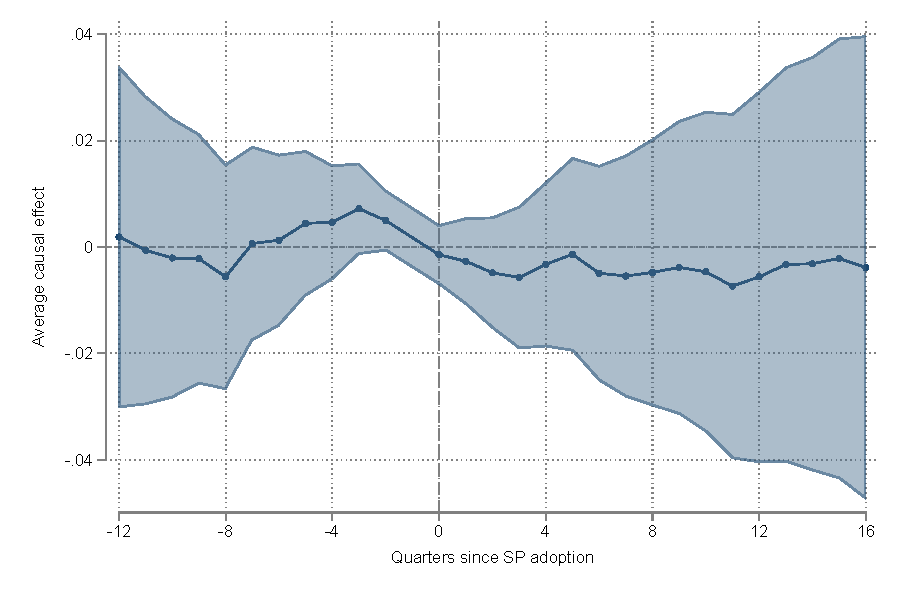
\includegraphics[width=\textwidth]{Figuras/did_event_flex_p_1.pdf}
    \end{subfigure}
        \begin{subfigure}{0.325\textwidth}
    \caption{Employees}
        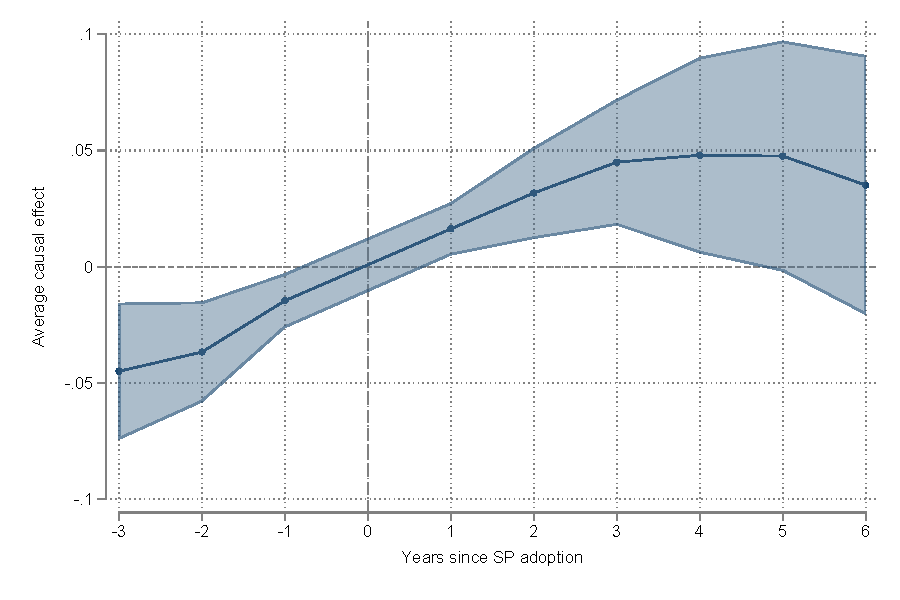
\includegraphics[width=\textwidth]{Figuras/did_event_flex_e_t.pdf}
    \end{subfigure}
  
  \end{center}
    \scriptsize 

%\textit{Scripts: }  \texttt{did\_es.do}
\end{figure}


\newpage

\subsection{Instrumental variables}

\vspace{.2in}
\begin{figure}[H]
     \caption{Clinics in MX}
    \label{map_clinics}
\begin{center}
\begin{subfigure}{0.45\textwidth}
\caption{Clinics in 2004}
        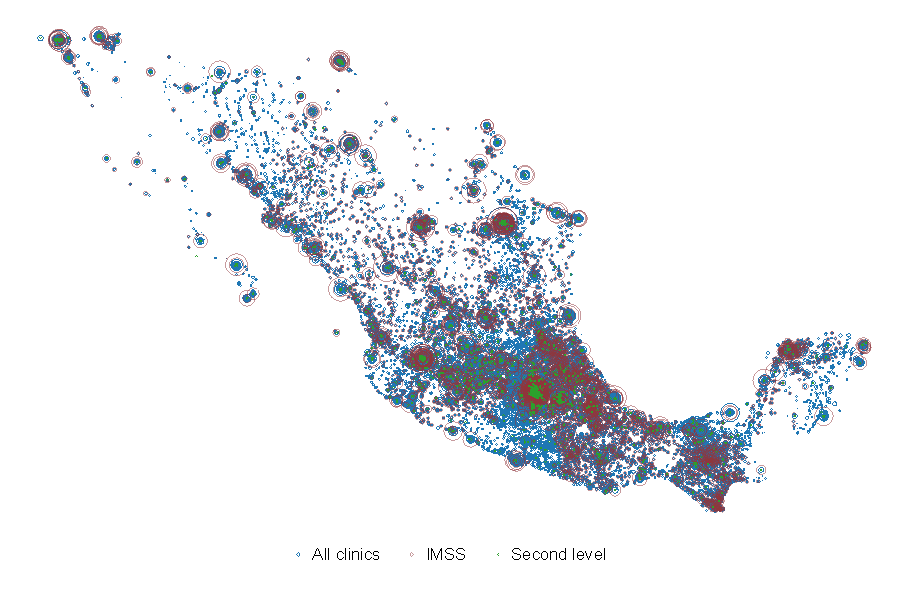
\includegraphics[width=\textwidth]{Figuras/map_clinics_04.pdf}
    \end{subfigure}
\begin{subfigure}{0.45\textwidth}
\caption{New clinics in 2007}
        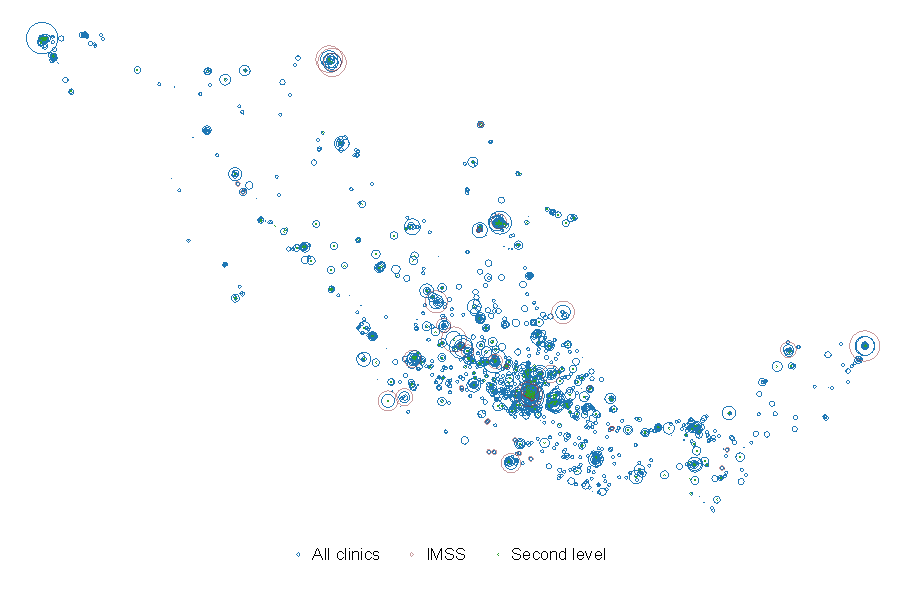
\includegraphics[width=\textwidth]{Figuras/map_clinics_07.pdf}
    \end{subfigure}    
  \end{center}
    \scriptsize 
%\textit{Scripts: }  \texttt{map_clinics.do}
\end{figure}




\vspace{.3in}
\begin{figure}[H]
     \caption{Trends of IMSS employment by terciles of the \# of clinics} \label{trends_clinics}
\begin{center}
    \begin{subfigure}{0.45\textwidth}
    \caption{Total employment}
        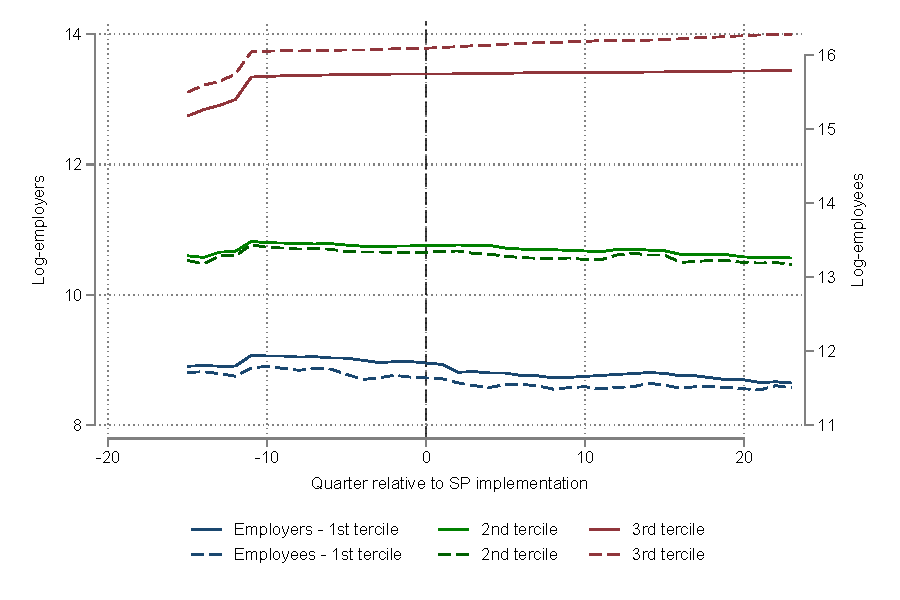
\includegraphics[width=\textwidth]{Figuras/trends_clinics_total.pdf}
    \end{subfigure}
    \begin{subfigure}{0.45\textwidth}
    \caption{Self-employed}
        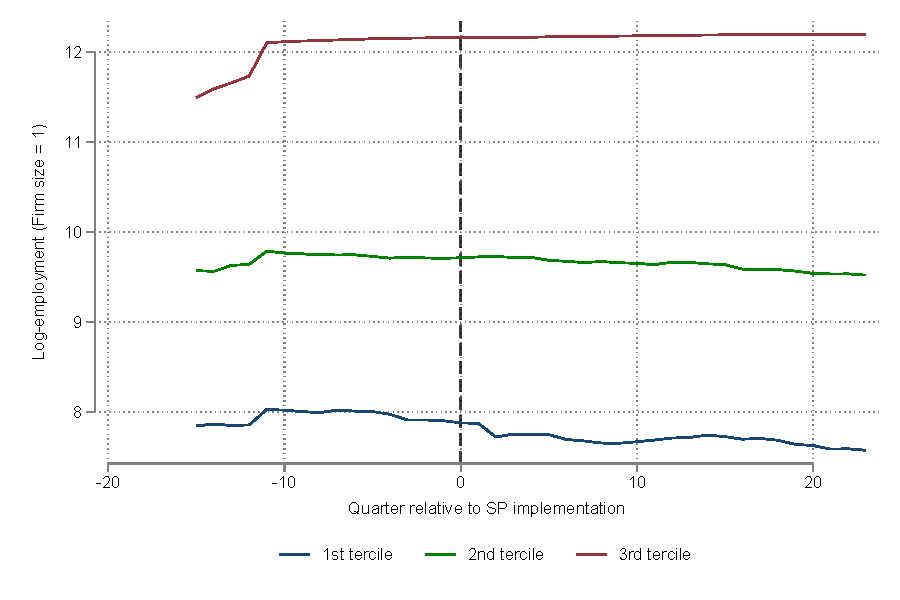
\includegraphics[width=\textwidth]{Figuras/trends_clinics_self.pdf}
    \end{subfigure}
  \end{center}
    
    \scriptsize 
%\textit{Scripts: }  \texttt{trends_emp_clinics.do}
\end{figure}




\begin{table}[H]
\caption{Pre-time trends (1-year)}
\label{pretime_trends}
\begin{center}
\resizebox{0.75\textwidth}{!}{
\scriptsize{% Table generated by Excel2LaTeX from sheet 'pretime_trends_instrument_4q'
\begin{tabular}{lccccccccccc}
\toprule
      & \multicolumn{2}{c}{Employer} &       & \multicolumn{2}{c}{Employee} &       & \multicolumn{2}{c}{Asalaried} &       & \multicolumn{2}{c}{Total wage mass} \\
\cmidrule{2-3}\cmidrule{5-6}\cmidrule{8-9}\cmidrule{11-12}      & (1)   & (2)   &       & (3)   & (4)   &       & (5)   & (6)   &       & (7)   & (8) \\
\midrule
\midrule
Log(Total \# clinics) & -0.019 &       &       & 0.083 &       &       & 0.085 &       &       & 0.037 &  \\
      & (0.033) &       &       & (0.071) &       &       & (0.071) &       &       & (0.057) &  \\
Log(\# IMSS clinics) & 0.015 &       &       & -0.016 &       &       & -0.032 &       &       & 0.058 &  \\
      & (0.016) &       &       & (0.032) &       &       & (0.033) &       &       & (0.046) &  \\
Log(\# 2nd level clinic) & -0.0030 &       &       & -0.016 &       &       & -0.018 &       &       & -0.033 &  \\
      & (0.018) &       &       & (0.032) &       &       & (0.032) &       &       & (0.035) &  \\
Log(\# 3rd level clinic) & 0.014 &       &       & -0.066** &       &       & -0.066** &       &       & -0.11** &  \\
      & (0.015) &       &       & (0.031) &       &       & (0.030) &       &       & (0.044) &  \\
Log(Total \# of rooms) & -0.070 &       &       & -0.11 &       &       & -0.095 &       &       & 0.0083 &  \\
      & (0.044) &       &       & (0.095) &       &       & (0.095) &       &       & (0.055) &  \\
Log(Total \# of beds) & -0.00081 &       &       & 0.028* &       &       & 0.018 &       &       & 0.025* &  \\
      & (0.0070) &       &       & (0.015) &       &       & (0.014) &       &       & (0.015) &  \\
PAN   & -0.0074 &       &       & -0.017 &       &       & -0.0049 &       &       & -0.0038 &  \\
      & (0.0067) &       &       & (0.015) &       &       & (0.015) &       &       & (0.020) &  \\
PRD   & 0     &       &       & 0     &       &       & 0     &       &       & 0     &  \\
      & (.)   &       &       & (.)   &       &       & (.)   &       &       & (.)   &  \\
\midrule
Log-population & -0.0081 & -0.061 &       & -0.33*** & -0.18** &       & -0.36*** & -0.17* &       & -0.69*** & -0.62*** \\
      & (0.050) & (0.038) &       & (0.12) & (0.085) &       & (0.13) & (0.092) &       & (0.15) & (0.098) \\
$\text{Luminosity}$ & 0.0041 & -0.0053 &       & 0.014** & 0.0028 &       & 0.017** & 0.0023 &       & 0.0063 & -0.026*** \\
      & (0.0034) & (0.0034) &       & (0.0073) & (0.0070) &       & (0.0081) & (0.0079) &       & (0.0088) & (0.0086) \\
$\text{Luminosity}^2$ & 0.000072 & 0.00012 &       & -0.00072** & -0.00062** &       & -0.00063** & -0.00058* &       & -0.000042 & 0.000080 \\
      & (0.00014) & (0.00014) &       & (0.00028) & (0.00028) &       & (0.00030) & (0.00030) &       & (0.00029) & (0.00029) \\
$\text{Luminosity}^3$ & -0.0000014 & -0.00000056 &       & 0.0000098*** & 0.000010*** &       & 0.0000084** & 0.0000096*** &       & 0.0000021 & 0.0000058* \\
      & (0.0000016) & (0.0000016) &       & (0.0000034) & (0.0000034) &       & (0.0000036) & (0.0000035) &       & (0.0000032) & (0.0000032) \\
Gender & -0.30*** & -0.37*** &       & -0.92*** & -1.01*** &       & -0.97*** & -1.10*** &       & -0.82*** & -1.07*** \\
      & (0.044) & (0.042) &       & (0.12) & (0.12) &       & (0.12) & (0.12) &       & (0.12) & (0.12) \\
Wage  & 0.00033*** & -0.00036*** &       & 0.0029*** & 0.0021*** &       & 0.0030*** & 0.0021*** &       & 0.0067*** & 0.0044*** \\
      & (0.00011) & (0.000088) &       & (0.00040) & (0.00027) &       & (0.00041) & (0.00028) &       & (0.00043) & (0.00028) \\
      &       &       &       &       &       &       &       &       &       &       &  \\
\midrule
Observations & 23200 & 23200 &       & 23200 & 23200 &       & 23402 & 23402 &       & 23464 & 23464 \\
R-sq  & 0.163 & 0.151 &       & 0.173 & 0.164 &       & 0.233 & 0.224 &       & 0.471 & 0.457 \\
F-statistics & 22.5  & 19.7  &       & 8.53  & 21.8  &       & 9.17  & 24.0  &       & 11.9  & 53.5 \\
p-value & 0.0013 &       &       & 0.090 &       &       & 0.081 &       &       & 0.15  &  \\
Municipality FE & \checkmark & \checkmark &       & \checkmark & \checkmark &       & \checkmark & \checkmark &       & \checkmark & \checkmark \\
LASSO selection &       & \checkmark &       &       & \checkmark &       &       & \checkmark &       &       & \checkmark \\
\bottomrule
\bottomrule
\end{tabular}%
}
}
\end{center}
 \scriptsize 
 In this table we test for the exclusion restriction of our instrument(s). This assumption states that the instruments are uncorrelated with outcome (employment) except that through its effect of SP implementation. To `test' for this assumption we estimate 
 $\log{\frac{y_{t+1}}{y_t}} = \alpha + \beta_kZ_{k,t} + \epsilon_{t}$ 
 in the pre-implementation periods.  Our hypothesis is that $\beta_k=0$. Odd-numbered columns estimates the previous equation and does not reject $H_0 : \beta_k = 0$. Even-numbered columns runs same specification but with variable selection using Lasso.
 
%\textit{Do file: } \texttt{iv\_sp.do}
\end{table}



\begin{figure}[H]
     \caption{First stage}
     \vspace{-.2in}
    \label{iv_fs}
\begin{center}
\begin{subfigure}{0.4\textwidth}
        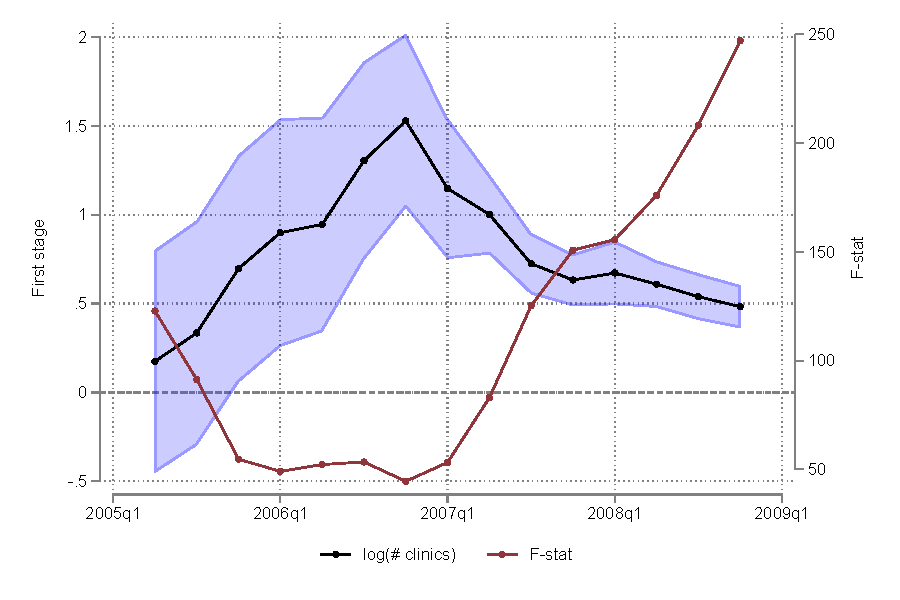
\includegraphics[width=\textwidth]{Figuras/IV_FS.pdf}
    \end{subfigure}
  \end{center}
  \vspace{-.15in}
    \scriptsize 
   This figure shows the F-statistic and an estimated coefficient for the first stage plotted for each quarter. Error are clustered at municipality level.
    
%\textit{Scripts: }  \texttt{iv_sp.do}
\end{figure}



\begin{figure}[H]
     \caption{Dynamic second stage}
     \vspace{-.2in}
    \label{iv_sp_dynamic}
\begin{center}
\begin{subfigure}{0.325\textwidth}
\caption{Employer}
        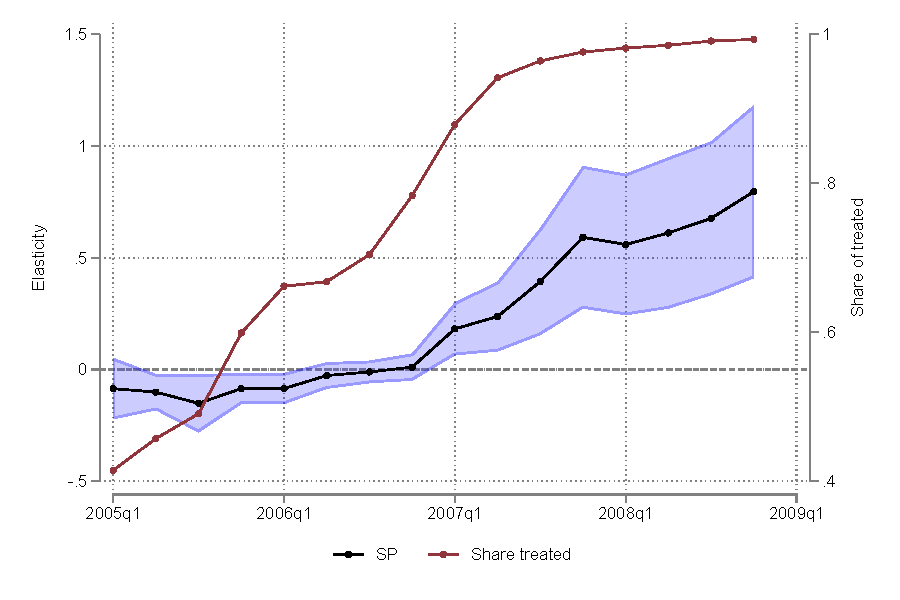
\includegraphics[width=\textwidth]{Figuras/IV_SP_p_t_.pdf}
    \end{subfigure}
\begin{subfigure}{0.325\textwidth}
\caption{Self-employed}
        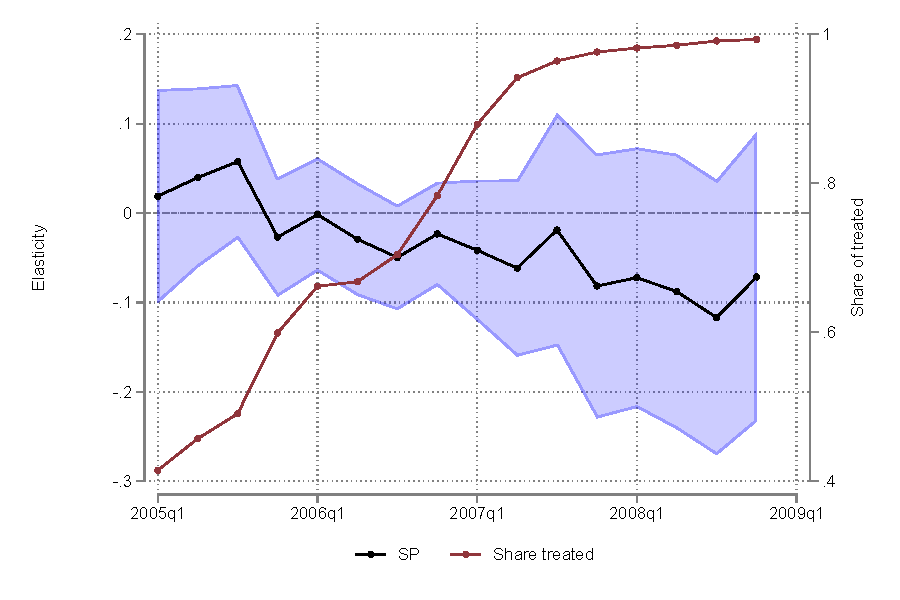
\includegraphics[width=\textwidth]{Figuras/IV_SP_p_1_.pdf}
    \end{subfigure}
\begin{subfigure}{0.325\textwidth}
\caption{Employee}
        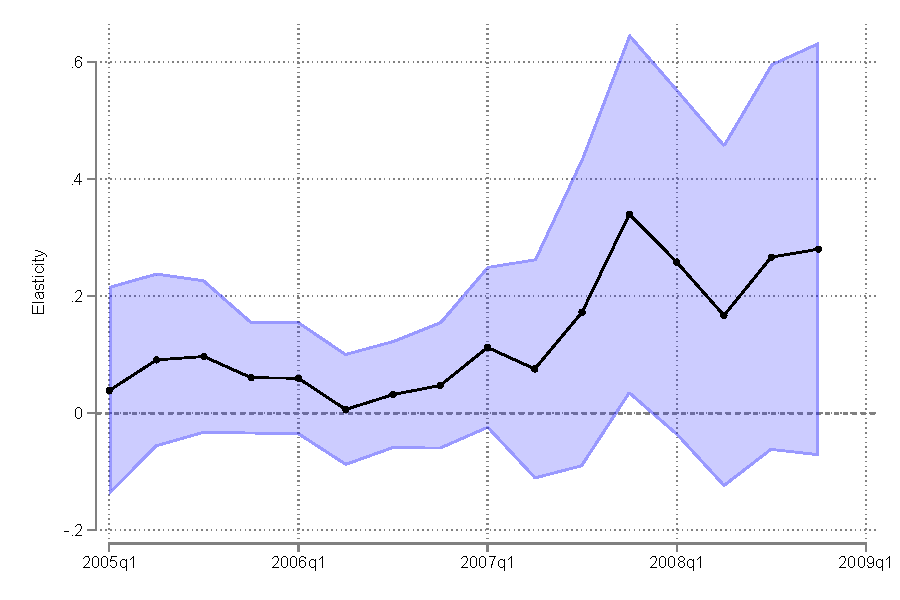
\includegraphics[width=\textwidth]{Figuras/IV_SP_e_t_.pdf}
    \end{subfigure}  
  \end{center}
  \vspace{-.15in}
    \scriptsize 
   This figure shows second stage separately for each quarter using the first stage from Figure \ref{iv_fs}. Error are clustered at municipality level.
    
%\textit{Scripts: }  \texttt{iv_sp.do}
\end{figure}

\vspace{2in}



\subsection{Difference of salaries for IMSS/no IMSS}

\begin{table}[H]
\caption{Salary changes}
\label{salary_changes}
\begin{center}
\resizebox{0.40\textwidth}{!}{
\scriptsize{% Table generated by Excel2LaTeX from sheet 'consequences_informal'
\begin{tabular}{lccccc}
\toprule
      & \multicolumn{2}{c}{[2005, 2010]} &       & \multicolumn{2}{c}{[2010, 2015]} \\
\cmidrule{2-3}\cmidrule{5-6}      & Log(hourly wage) & Weekly hours &       & Log(hourly wage) & Weekly hours \\
\midrule
      & (1)   & (2)   &       & (3)   & (4) \\
\midrule
\midrule
No IMSS & -0.23*** & -5.79*** &       & -0.15*** & -6.50*** \\
      & (0.00) & (0.00) &       & (0.00) & (0.00) \\
Woman & -0.12*** & -7.33*** &       & -0.06*** & -7.21*** \\
      & (0.00) & (0.00) &       & (0.00) & (0.00) \\
Age   & -0.00*** & 0.01*** &       & -0.00*** & 0.00*** \\
      & (0.00) & (0.00) &       & (0.00) & (0.00) \\
Years of schooling & 0.01*** & 0.04*** &       & -0.01*** & 0.03*** \\
      & (0.00) & (0.00) &       & (0.00) & (0.00) \\
Married & 0.25*** & 1.59*** &       & 0.23*** & 1.50*** \\
      & (0.00) & (0.00) &       & (0.00) & (0.00) \\
      &       &       &       &       &  \\
\midrule
Obs   & 3.376e+06 & 3.376e+06 &       & 3.991e+06 & 3.991e+06 \\
Population & 887,534,856 & 887,534,856 &       & 1169577977 & 1169577977 \\
R-squared & 0.18  & 0.16  &       & 0.14  & 0.17 \\
Dep var mean & 2.272 & 41.29 &       & 2.213 & 41.21 \\
Municipality $\times$ Date FE & \checkmark & \checkmark &       & \checkmark & \checkmark \\
Occupation FE & \checkmark & \checkmark &       & \checkmark & \checkmark \\
\bottomrule
\bottomrule
\end{tabular}%
}
}
\end{center}
\scriptsize 
% \textit{Do file: } \texttt{consequences\_informal.do}
\end{table}


\newpage 




\end{document}

